\documentclass[10pt,a4paper,twocolumn]{article}

\usepackage[utf8]{inputenc}
\usepackage[T1]{fontenc}
\usepackage[spanish,es-nodecimaldot]{babel}
\usepackage{lmodern}
\usepackage{microtype}
\usepackage{amsmath}
\usepackage{amssymb}
\usepackage{geometry}
\usepackage{booktabs}
\usepackage{tabularx}
\usepackage{array}
\usepackage{enumitem}
\usepackage{siunitx}
\usepackage{graphicx}
\usepackage{float}
\usepackage{dblfloatfix}
\usepackage{placeins}
\usepackage{xcolor}
\usepackage{hyperref}

\geometry{margin=2.5cm}
\setlength{\columnsep}{0.7cm}
% Evita que LaTeX estire el espacio vertical para igualar columnas cortas:
% con figuras grandes eso dejaba huecos enormes entre subsecciones.
\raggedbottom
\setlist[itemize]{itemsep=0.2em}
\sisetup{output-decimal-marker={,}}
\newcolumntype{Y}{>{\raggedright\arraybackslash}X}
\hypersetup{
    colorlinks=true,
    linkcolor=black,
    citecolor=black,
    urlcolor=blue
}
\graphicspath{{../../Propuesta Urucom/Imagenes/}{../latex-historial/figuras/}{figuras/interfaces/}{figuras/comerciales/}{figuras/acondicionamiento/}{figuras/transductores/}{figuras/casos_estudio/}}

\title{Diseño e implementación de un sistema electrónico multicanal del tipo IoT para
caracterización geotécnica del suelo mediante ondas sísmicas\\[0.5em]
\large Proyecto final de carrera -- Primera presentación}
\author{Elías David Álvarez Martínez}
\date{}

\begin{document}

\maketitle

% Los \FloatBarrier explícitos entre secciones eran redundantes con la opción
% [section] de placeins y forzaban cortes de columna con huecos grandes.
\section{Utilidad del modelado del subsuelo, métodos disponibles y brecha de acceso}
\label{sec:problema-modelado}

\subsection{El problema no es abstracto: se toman decisiones sobre un medio que no se ve}

Toda obra se apoya en un material cuya estructura no puede observarse directamente en
su totalidad. El suelo no es una pieza fabricada y uniforme: su composición, rigidez,
compactación, saturación y espesor cambian con la profundidad y también entre puntos
cercanos. Por eso, antes de construir, rehabilitar o estudiar una obra aparecen
preguntas concretas:

\begin{itemize}
    \item ¿A qué profundidad cambia significativamente la rigidez del terreno?
    \item ¿Existe una capa blanda, un relleno, una cavidad o un contacto con roca?
    \item ¿El perfil observado en un sondeo representa realmente todo el sitio?
    \item ¿Cómo puede amplificar el terreno una vibración o un movimiento sísmico?
    \item ¿Dónde conviene realizar ensayos adicionales antes de tomar una decisión?
\end{itemize}

Modelar el subsuelo significa transformar observaciones parciales en una
representación de capas o zonas con propiedades mecánicas estimadas. El modelo no es
una fotografía exacta del terreno; es una hipótesis cuantitativa que debe ser compatible
con las mediciones, la geología conocida y la resolución del método empleado.

En este trabajo interesa especialmente la velocidad de onda de corte, $V_S$, porque se
relaciona con el módulo de corte a pequeñas deformaciones mediante

\begin{equation}
    G_{\max}=\rho V_S^2,
\end{equation}

donde $\rho$ es la densidad del material. Un perfil $V_S(z)$ permite reconocer cambios
de rigidez con la profundidad y aporta una entrada fundamental para la clasificación
sísmica y el análisis de respuesta de sitio~\cite{Kramer1996,Foti2014}. Cuando se
repiten perfiles a lo largo de una línea o sobre una grilla, la información deja de ser
puramente puntual y puede convertirse en una sección 2D o en un modelo 3D.

La utilidad no está, entonces, en ``medir una señal sísmica''. La señal es el dato
crudo; el producto de ingeniería es un modelo del subsuelo con alcance, supuestos e
incertidumbre declarados.

\subsection{Física de las ondas sísmicas: ondas de cuerpo y ondas de superficie}

Toda perturbación mecánica del suelo se propaga mediante dos familias de ondas
elásticas. Las \textbf{ondas de cuerpo} viajan a través del volumen del medio: las ondas
P (primarias, de compresión) desplazan la partícula en la misma dirección de
propagación, mientras que las ondas S (secundarias, de corte) la desplazan
perpendicularmente a ella. Sus velocidades dependen de los módulos elásticos y de la
densidad $\rho$,

\begin{equation}
    V_P=\sqrt{\frac{K+\frac{4}{3}G}{\rho}},
    \qquad
    V_S=\sqrt{\frac{G}{\rho}},
\end{equation}

con $K$ el módulo volumétrico y $G$ el módulo de corte. $V_S$ no depende de $K$ y, a
diferencia de $V_P$, no se propaga en fluidos porque éstos no resisten esfuerzo de
corte; por eso $V_S$ es el indicador más directo de la rigidez al corte del esqueleto del
suelo, la magnitud que interesa a lo largo de esta tesis.

Cuando el semiespacio tiene una superficie libre aparecen además las \textbf{ondas de
superficie}, producto de la interferencia entre ondas P y SV reflejadas
repetidamente cerca de esa frontera. La onda Rayleigh resulta de esa interferencia: cada
partícula describe una trayectoria elíptica retrógrada en el plano vertical que contiene
la dirección de propagación, con amplitud que decae aproximadamente de forma exponencial
con la profundidad y geométricamente como $1/\sqrt{r}$ con la distancia a la fuente, en
lugar de $1/r$ o $1/r^2$ como las ondas de cuerpo. Esa atenuación geométrica más lenta
explica por qué, a pocos metros de una fuente impulsiva en superficie, la energía
Rayleigh domina el registro: puede transportar hasta dos tercios de la energía sísmica
total generada por el impacto~\cite{Foti2014,Kramer1996}. La onda Love, en cambio,
resulta del atrapamiento de ondas SH en una capa superficial de menor velocidad y
produce movimiento horizontal transversal a la propagación, sin componente vertical; por
eso no se registra con geófonos verticales convencionales.

Esta jerarquía energética y geométrica es la razón física por la que un MASW activo con
geófonos verticales, aunque sólo observa una fracción del campo de ondas completo,
captura la componente más intensa y más directamente vinculada a $V_S$: la Rayleigh
vertical. Las secciones siguientes explotan justamente esa relación entre dispersión de
Rayleigh y estructura de $V_S(z)$.

\subsection{Casos reales: de la medición a una decisión}

Los siguientes casos muestran que el modelado sísmico del subsuelo ya se utiliza para
problemas de construcción, rehabilitación, clasificación de sitio e investigación. No
son demostraciones de laboratorio: en todos ellos la información obtenida responde a
una necesidad concreta del sitio.

\textbf{CentrePort, Wellington.} El puerto de Wellington, Nueva Zelanda, sufrió
licuefacción, desplazamiento lateral y daños estructurales durante el terremoto de
Kaik\={o}ura ($M_w=7{,}8$). Se combinaron 114 mediciones HVSR con MASW activo y arreglos
pasivos MAM para obtener, en seis ubicaciones, perfiles $V_S$ de más de \SI{200}{\meter}
de profundidad y un mapa de período fundamental de sitio, usados para explicar por qué
la amplificación varió en distancias cortas y para orientar medidas de
mitigación~\cite{Vantassel2018}. El caso muestra que combinar métodos activos, pasivos y
de sondeo produce una interpretación más fuerte que cualquiera por separado.

\textbf{Mina abandonada en Colorado.} Antes de construir un estanque industrial sobre
una antigua mina de oro, se adquirieron 40 perfiles MASW para investigar los primeros
\SIrange{9}{15}{\meter} del subsuelo y localizar pozos colapsados y labores someras mal
documentadas. El mapa de zonas anómalas resultante se usó para concentrar la
investigación adicional y el movimiento de suelo donde el riesgo era mayor, sin pretender
``fotografiar'' la geometría exacta de cada labor~\cite{Crook2017}.

\textbf{Campus de Delhi Technological University.} Con un sismógrafo comercial PASI
GEA24 de 24 canales, geófonos de \SI{4.5}{\hertz} y maza como fuente, se realizaron 30
ensayos MASW en seis sectores del campus, obteniendo una $V_S$ media de
\SI{285}{\meter\per\second} y clasificando el sitio como clase D según NEHRP. Este caso
conecta directamente una aplicación real con uno de los equipos comerciales analizados
más adelante, mostrando el flujo industrial completo: arreglo, fuente, adquisición,
dispersión, inversión y clasificación~\cite{Gautam2020}.

\textbf{Metro Manila.} En tres sitios se comparó $V_{S,30}$ obtenida por vía geotécnica
(SPT y calidad de roca) con la obtenida por MASW. Aunque los valores numéricos difirieron,
ambos caminos produjeron la misma clasificación sísmica NEHRP, mostrando que MASW no
reemplaza al SPT sino que lo complementa: el sondeo aporta muestra y detalle local, la
geofísica aporta cobertura y una estimación dinámica~\cite{Monjardin2023}.

\textbf{Construcción y mantenimiento de carreteras.} MASW se emplea rutinariamente en
dos extremos de la ingeniería vial: ensayos rápidos de poca profundidad
(\SI{30}{\centi\meter}) para controlar la rigidez de cada capa del pavimento
---asfáltica, base, subbase y subrasante--- tras la compactación, y estudios de mayor
profundidad (\SI{30}{\meter}) durante la planificación de una carretera nueva, donde
interesa el contacto con el lecho rocoso. Park et al. documentan casos de ambos extremos
ejecutados durante el inicio, el cierre y el mantenimiento de una obra
vial~\cite{Park2018Roads}; esta misma aplicación motivó, en una propuesta de
financiación previa a este proyecto, evaluar MASW como alternativa no destructiva para
caracterización de pavimentos y suelos de fundación viales~\cite{PINV01317}.

Estos seis casos no agotan el abanico de usos: Park resume, además, el mapeo de
interfaces de lecho rocoso, la clasificación sísmica de sitio mediante $V_{S,30}$, la
evaluación de licuefacción y la caracterización previa a la construcción de plantas que
alojan maquinaria vibratoria de gran amplitud, como centrales de generación de
energía~\cite{Park2013}.

\begin{table}[ht]
\centering
\small
\caption{Qué demuestra cada caso de estudio.}
\begin{tabularx}{\textwidth}{@{}>{\raggedright\arraybackslash}p{0.19\textwidth} Y Y@{}}
\toprule
\textbf{Caso} & \textbf{Pregunta práctica} & \textbf{Resultado utilizable} \\
\midrule
CentrePort & ¿Por qué varió la amplificación y qué profundidad debe incluir el modelo? & Mapa de período de sitio y perfiles profundos de rigidez y roca para análisis de respuesta. \\
Mina de Colorado & ¿Dónde pueden existir labores colapsadas antes de construir? & Mapa de zonas débiles o vacíos para orientar investigación y movimiento de suelo. \\
Campus de Delhi & ¿Cómo varía la rigidez entre sectores del campus? & Perfiles $V_S$ y clasificación sísmica a partir de 30 ensayos. \\
Metro Manila & ¿Son compatibles la investigación geotécnica y la geofísica? & Clasificación NEHRP consistente mediante SPT/RQD y MASW. \\
Carreteras & ¿Cumple cada capa del pavimento la rigidez de diseño? & Control de calidad rápido en obra y estudio de profundidad en la planificación vial. \\
\bottomrule
\end{tabularx}
\end{table}

\subsection{Métodos disponibles: cada uno observa una parte distinta del problema}

No existe un método universalmente superior. La elección depende de la propiedad que
se desea conocer, la profundidad, la resolución, la cobertura, el acceso al sitio y el
nivel de incertidumbre aceptable. Una primera división separa los ensayos que requieren
penetrar o perforar el terreno de aquellos que infieren propiedades desde la superficie.

\begin{table}[ht]
\centering
\footnotesize
\caption{Comparación funcional de métodos de caracterización.}
\begin{tabularx}{\textwidth}{@{}>{\raggedright\arraybackslash}p{0.13\textwidth} >{\raggedright\arraybackslash}p{0.18\textwidth} Y Y@{}}
\toprule
\textbf{Método} & \textbf{Información principal} & \textbf{Fortaleza} & \textbf{Limitación relevante} \\
\midrule
SPT & Resistencia a penetración y muestra alterada & Práctica extendida, contacto directo y correlaciones geotécnicas conocidas & Información puntual; requiere sondeo; $V_S$ se obtiene sólo mediante correlaciones empíricas \\
CPT/CPTu & Resistencia de punta, fricción y, con CPTu, presión de poros & Perfil casi continuo y buena resolución estratigráfica & Intrusivo; no recupera muestra; dificultad en gravas o materiales muy duros \\
Downhole / crosshole & Tiempos de viaje y $V_P$/$V_S$ en profundidad & Alta resolución local y referencia valiosa para validar otros métodos & Requiere uno o varios pozos y representa un volumen limitado \\
Refracción / tomografía & Velocidad de primeras llegadas, usualmente $V_P$ & Buena lectura lateral de contactos y profundidad a roca & Las capas de baja velocidad bajo capas rígidas pueden quedar ocultas; no entrega directamente $V_S$ salvo configuración específica \\
MASW activo & Curva de dispersión y perfil $V_S(z)$ & No invasivo, multicanal y repetible; permite perfiles 1D y secciones pseudo-2D & Requiere fuente, arreglo sincronizado e inversión; existe compromiso entre resolución y profundidad \\
MAM / ReMi / SPAC & Dispersión del ruido ambiental & Extiende la investigación a frecuencias bajas y mayores profundidades sin fuente controlada & Depende del campo de ruido, la geometría y registros más largos \\
HVSR & Frecuencia o período fundamental del sitio & Una estación triaxial y despliegue rápido & Por sí solo no determina un perfil $V_S$ único \\
ERT & Distribución de resistividad eléctrica & Sensible a saturación, arcillas, cavidades y cambios litológicos & La resistividad no es una medida directa de rigidez mecánica \\
\bottomrule
\end{tabularx}
\end{table}

SPT, CPT, downhole y crosshole son valiosos porque entregan información de contacto
directo, pero describen bien su entorno inmediato y la extrapolación entre sondeos puede
ocultar variaciones laterales; por eso la pregunta correcta no es ``¿sondeo o
geofísica?'', sino cómo usar los sondeos para anclar una medición que cubra un volumen
mayor, como en CentrePort, donde los datos CPT y de perforación restringieron la
parametrización de la inversión de ondas superficiales~\cite{Vantassel2018}. La
refracción, la resistividad y las ondas superficiales, en cambio, intercambian ese
contacto directo por cobertura espacial: permiten estudiar líneas o superficies sin
perforar cada punto, pero el resultado se obtiene mediante un problema inverso donde
varias estructuras pueden explicar datos similares. La geofísica no es, entonces, una
``radiografía'' perfecta; su utilidad está en aportar información espacial y dinámica
que los ensayos puntuales no entregan con la misma facilidad.

\subsection{Por qué las ondas superficiales y por qué MASW}

Las ondas Rayleigh son dispersivas en un medio estratificado: componentes de distinta
longitud de onda muestrean volúmenes diferentes del subsuelo y se propagan con
velocidades de fase distintas, y esa dependencia contiene información sobre la
distribución de $V_S$. El procedimiento MASW activo explota esa propiedad en tres
etapas: \textbf{adquisición} (una fuente controlada genera ondas que un arreglo de
receptores registra simultáneamente), \textbf{análisis de dispersión} (las señales se
transforman al dominio frecuencia--velocidad para identificar las curvas modales) e
\textbf{inversión} (se buscan perfiles estratificados cuya dispersión teórica sea
compatible con la observada). MASW evolucionó respecto de SASW al pasar de pares de
receptores a un registro multicanal simultáneo, lo que facilita separar energía
coherente, reduce ambigüedades de fase y aumenta la productividad de
campo~\cite{Park1999}; los métodos pasivos MAM, ReMi o SPAC no compiten con el activo,
sino que pueden extender la curva hacia frecuencias más bajas y mayores profundidades.

Se eligió MASW activo para este proyecto porque permite generar una excitación
repetible, trabajar con geometría conocida y evaluar directamente la cadena instrumental
multicanal desarrollada, sin eliminar sus limitaciones: la profundidad depende de las
longitudes de onda observadas con relación señal--ruido suficiente; la apertura, el
espaciamiento y el \emph{offset} condicionan la banda válida; los modos superiores
pueden confundirse con el fundamental; la inversión es no única; y errores de fase entre
canales se traducen directamente en errores de velocidad de fase. El proyecto
InterPACIFIC y sus guías derivadas mostraron que los métodos de ondas superficiales
producen resultados reproducibles entre equipos cuando se documentan geometría, banda
válida, procesamiento e incertidumbre, pero que el perfil final depende fuertemente de
la parametrización de la inversión~\cite{Foti2018}: el instrumento debe entregar datos
sincronizados y trazables de calidad conocida, sin poder eliminar por sí solo la no
unicidad del subsuelo.

\subsection{De la señal medida al modelo \texorpdfstring{$V_S(z)$}{Vs(z)}: física y ecuaciones}

La cadena que suele resumirse como

\begin{center}
$V_{R,\mathrm{aparente}}\longrightarrow V_S\longrightarrow\text{modelo}$
\end{center}

contiene en realidad dos problemas distintos. Primero se estima, a partir de las
señales multicanal, cómo cambia la velocidad de fase de las ondas Rayleigh con la
frecuencia. Después se buscan las propiedades de un medio estratificado que puedan
producir esa dispersión. Esta distinción es esencial: en un suelo formado por capas no
se mide directamente la $V_S$ de una profundidad determinada.

\subsubsection{Del registro espacio--tiempo a la velocidad de fase aparente}

Sea $u(x_j,t)$ el desplazamiento o, en la práctica, la señal proporcional a velocidad
registrada por el geófono ubicado en $x_j$. Para cada canal se calcula la transformada
temporal de Fourier

\begin{equation}
    U(x_j,\omega)=\int_{-\infty}^{\infty}u(x_j,t)
    e^{i\omega t}\,\mathrm{d}t
    =A(x_j,\omega)e^{i\phi(x_j,\omega)}.
\end{equation}

Si una componente de frecuencia $f=\omega/(2\pi)$ se propaga como una onda plana, su
fase cambia aproximadamente como $\phi(x,\omega)=\phi_0-kx$, con número de onda
$k=\omega/c_R$. Entre dos receptores separados una distancia $\Delta x$ se obtendría
entonces

\begin{equation}
    c_{R,\mathrm{aparente}}(f)
    =\frac{\omega\,\Delta x}{|\Delta\phi(f)|}
    =\frac{2\pi f\,\Delta x}{|\Delta\phi(f)|}.
    \label{eq:velocidad-fase-dos-canales}
\end{equation}

El problema práctico de esta expresión es que la fase está definida módulo $2\pi$,
puede contaminarse con ruido y puede contener simultáneamente varios modos. MASW utiliza
todos los canales para reducir esa ambigüedad. En el método de desplazamiento de fase
se prueba una velocidad $c$ y se corrige la fase esperada en cada posición. Una forma
normalizada del espectro es~\cite{Park1998}

\begin{equation}
    S(\omega,c)=\frac{1}{N}\left|
    \sum_{j=1}^{N}
    \frac{U(x_j,\omega)}{|U(x_j,\omega)|}
    \exp\!\left(i\frac{\omega x_j}{c}\right)
    \right|.
    \label{eq:phase-shift}
\end{equation}

Cuando la velocidad ensayada coincide con la velocidad de fase de una onda presente,
las contribuciones de los receptores se alinean y $S$ presenta un máximo. Al seleccionar
esos máximos para cada frecuencia se obtiene la curva observada

\begin{equation}
    c_R^{\mathrm{obs}}(f)=\operatorname*{arg\,max}_{c}S(2\pi f,c).
\end{equation}

Se la denomina velocidad de fase \emph{aparente} porque se infiere desde un arreglo
finito y puede incluir efectos de ruido, modos, geometría y variación lateral. Bajo la
aproximación de estratos horizontales representa la dispersión modal de Rayleigh que se
utilizará en la inversión.

\subsubsection{Frecuencia, longitud de onda y profundidad}

Cada punto de la curva tiene asociada una longitud de onda

\begin{equation}
    \lambda_R(f)=\frac{c_R(f)}{f}.
    \label{eq:longitud-onda}
\end{equation}

Las longitudes de onda cortas concentran mayor sensibilidad cerca de la superficie;
las largas involucran un volumen más profundo. No existe, sin embargo, una igualdad
universal del tipo $z=\lambda/2$: cada medición posee una función de sensibilidad
distribuida y solapada con la de otras frecuencias. La regla de una fracción de la
longitud de onda sirve para diseñar e interpretar preliminarmente el ensayo, no para
asignar cada velocidad a una profundidad exacta.

Por ejemplo, un máximo de dispersión de \SI{240}{\meter\per\second} a
\SI{20}{\hertz} corresponde a $\lambda_R=\SI{12}{\meter}$. Ese dato restringe la
combinación de propiedades de las capas someras sensibles a esa longitud de onda; no
significa que $V_S$ a \SI{6}{\meter} sea \SI{240}{\meter\per\second}. Un punto de
\SI{500}{\meter\per\second} a \SI{5}{\hertz}, en cambio, tiene
$\lambda_R=\SI{100}{\meter}$ y aporta información integrada de un volumen mucho más
profundo.

\subsubsection{Relación física entre \texorpdfstring{$c_R$ y $V_S$}{cR y Vs}}

En un semiespacio elástico, homogéneo e isótropo, la velocidad de Rayleigh se relaciona
con $V_S$ y $V_P$. Si $\xi=c_R/V_S$ y $\kappa=(V_S/V_P)^2$, la raíz física satisface

\begin{equation}
    \xi^6-8\xi^4+(24-16\kappa)\xi^2-16(1-\kappa)=0.
    \label{eq:rayleigh-homogeneo}
\end{equation}

Para una relación de Poisson $\nu=0{,}25$, $\kappa=1/3$ y
$c_R\simeq0{,}9194V_S$~\cite{Xia1999}. Sólo bajo ese modelo homogéneo podría utilizarse
la aproximación $V_S\simeq c_R/0{,}9194$. Así, para el ejemplo anterior se obtendría
$V_S\simeq\SI{261}{\meter\per\second}$, pero sería la velocidad de un semiespacio
equivalente, no el valor de una capa a una profundidad particular.

En un terreno estratificado, las condiciones de continuidad de esfuerzos y
desplazamientos en cada interfaz producen una ecuación característica cuyos ceros
dependen de la frecuencia y del modelo completo:

\begin{equation}
    F\!\left(f,c_R;\boldsymbol{V}_S,\boldsymbol{V}_P,
    \boldsymbol{\rho},\boldsymbol{h}\right)=0.
    \label{eq:forward-rayleigh}
\end{equation}

Aquí $\boldsymbol{h}$ contiene los espesores y $\boldsymbol{V}_S$,
$\boldsymbol{V}_P$ y $\boldsymbol{\rho}$ las propiedades de cada estrato. Para cada
frecuencia, las raíces de la ecuación~\eqref{eq:forward-rayleigh} son las velocidades
de fase teóricas de los distintos modos. En el rango habitual de ingeniería la
dispersión de Rayleigh es especialmente sensible a $V_S$ y, después, a los espesores;
por eso $V_P$ y $\rho$ suelen fijarse o restringirse con información auxiliar
~\cite{Xia1999}.

\subsubsection{De la curva de dispersión a una familia de modelos}

La inversión parte de los datos
$\boldsymbol{d}=[c_R^{\mathrm{obs}}(f_1),\ldots,c_R^{\mathrm{obs}}(f_M)]$ y propone un
modelo

\begin{equation}
\begin{split}
    \boldsymbol{m}=[&h_1,\ldots,h_{L-1},
    V_{S,1},\ldots,V_{S,L},\\
    &V_{P,1},\ldots,V_{P,L},
    \rho_1,\ldots,\rho_L].
\end{split}
\end{equation}

Un solucionador directo calcula
$\boldsymbol{g}(\boldsymbol{m})=\boldsymbol{c}_R^{\mathrm{calc}}$ mediante la
ecuación~\eqref{eq:forward-rayleigh}. La inversión modifica el modelo para minimizar,
por ejemplo,

\begin{equation}
    \Phi(\boldsymbol{m})=
    \left\|\boldsymbol{W}_d
    [\boldsymbol{d}-\boldsymbol{g}(\boldsymbol{m})]\right\|_2^2
    +\lambda\,R(\boldsymbol{m}),
    \label{eq:objetivo-inversion}
\end{equation}

donde $\boldsymbol{W}_d$ pondera cada dato según su incertidumbre y
$R(\boldsymbol{m})$ penaliza modelos incompatibles con restricciones elegidas, por
ejemplo variaciones excesivamente abruptas. En una inversión linealizada, la corrección
puede expresarse como

\begin{equation}
    (\boldsymbol{J}^{T}\boldsymbol{W}\boldsymbol{J}+\lambda\boldsymbol{L}^{T}
    \boldsymbol{L})\,\Delta\boldsymbol{m}
    =\boldsymbol{J}^{T}\boldsymbol{W}
    [\boldsymbol{d}-\boldsymbol{g}(\boldsymbol{m})],
\end{equation}

con $J_{ij}=\partial c_R(f_i)/\partial m_j$. El proceso se repite con
$\boldsymbol{m}_{k+1}=\boldsymbol{m}_k+\Delta\boldsymbol{m}$, o se reemplaza por una
búsqueda global; aquí $\boldsymbol{W}=\boldsymbol{W}_d^T\boldsymbol{W}_d$. En ambos
casos la salida honesta no es una única ``fotografía'', sino
un conjunto de modelos aceptables y sus bandas de variación.

Una vez estimado el perfil $V_S(z)$ pueden calcularse magnitudes de ingeniería. Para
capas que completan los primeros \SI{30}{\meter},

\begin{equation}
    V_{S,30}=\frac{30}{\displaystyle\sum_i h_i/V_{S,i}},
    \qquad
    G_{\max,i}=\rho_i V_{S,i}^{2}.
\end{equation}

La cadena física completa queda, por tanto,

\begin{center}
\small
$u_j(t)\rightarrow U_j(f)\rightarrow S(f,c)\rightarrow
c_R^{\mathrm{obs}}(f)\rightarrow
\text{inversión estratificada}\rightarrow
\{h_i,V_{S,i},V_{P,i},\rho_i\}\rightarrow V_S(z),V_{S,30},G_{\max}$.
\end{center}

Esto también explica por qué la instrumentación importa: error de fase entre canales,
una banda recortada por el transductor o una geometría mal documentada alteran la curva
de dispersión antes de que el algoritmo de inversión pueda intervenir.

\subsection{Soluciones comerciales: evidencia de interés industrial}

La existencia de varias familias de sismógrafos profesionales confirma que la
adquisición sísmica somera no es un problema puramente académico. Los fabricantes han
invertido en mejorar exactamente los aspectos que aparecen en campo: resolución y rango
dinámico, sincronización, control sencillo, autonomía, escalabilidad y reducción de
cableado.

Por eso no resulta correcto presentar esta parte como ``problemas de los MASW
comerciales''. Son soluciones maduras y, en varios casos, muy capaces. Lo que interesa
es observar qué arquitectura adopta cada una y qué necesidad industrial demuestra.

\begin{table}[ht]
\centering
\footnotesize
\caption{Soluciones comerciales y señal de demanda industrial. Las prestaciones provienen de las páginas oficiales de los fabricantes.}
\begin{tabularx}{\textwidth}{@{}>{\raggedright\arraybackslash}p{0.16\textwidth} >{\raggedright\arraybackslash}p{0.22\textwidth} Y Y@{}}
\toprule
\textbf{Producto} & \textbf{Arquitectura} & \textbf{Qué resuelve} & \textbf{Qué demuestra} \\
\midrule
Geometrics GeodeFlex & 24 canales analógicos centralizados; control web; Wi-Fi en versión Core; GPS integrado & Adquisición simultánea de 24 bits, operación desde PC, tableta o teléfono y registro autónomo & La interfaz web y la sincronización forman parte del valor industrial, no son accesorios \\
PASI GEA24 & Sismógrafo compacto de 24 canales conectado por USB a una computadora; ampliable a 48 & Portabilidad, alimentación USB y uso multipropósito: MASW, Vs30, refracción, tomografía y pozo & Existe demanda por una plataforma compacta que reutilice la misma adquisición en varios métodos \\
DMT SUMMIT X One & Unidades remotas distribuidas sobre un cable ligero de dos conductores para datos y energía & Geometrías flexibles, despliegue rápido y escalabilidad desde más de 24 hasta miles de canales & Reducir el cableado y distribuir la adquisición tiene valor operativo real \\
Geometrics Atom-3C & Unidades triaxiales autónomas, temporizadas por GPS, sin cable de tendido; descarga por Wi-Fi & Adquisición pasiva prolongada sin fuente, computadora ni interconexión entre estaciones & La autonomía y la eliminación de cables son suficientemente valiosas para justificar una familia específica de producto \\
\bottomrule
\end{tabularx}
\end{table}

\textbf{Geometrics GeodeFlex} integra 24 canales de 24 bits con controlador Linux, GPS,
Wi-Fi y una aplicación web operable desde computadora, tableta o teléfono, incluido
registro autónomo sincronizado por GPS para ensayos pasivos~\cite{GeometricsGeodeFlex}.
El Wi-Fi simplifica el control, pero los 24 geófonos y el disparo activo siguen
cableados: demuestra que una interfaz web moderna mejora la operación de campo incluso
sobre una arquitectura de adquisición centralizada.

\textbf{PASI GEA24} compacta 24 canales de 24 bits en una unidad alimentada y controlada
por USB desde una computadora, ampliable a 48 canales, y orientada a MASW, refracción,
tomografía, downhole, crosshole y $V_{S,30}$~\cite{PASIGEA24}; el caso de Delhi confirma
su uso efectivo en campo~\cite{Gautam2020}. Conserva los cables sísmicos tradicionales,
pero reduce volumen y elimina la batería independiente: una optimización clara del
esquema centralizado.

\textbf{DMT SUMMIT X One} desplaza la conversión hacia unidades remotas conectadas sobre
un cable ligero de dos conductores que distribuye energía y datos, con configuraciones
desde 24 hasta miles de canales y registro continuo para pasivo~\cite{DMTSummitXOne}.
Muestra que distribuir nodos no obliga a eliminar todo cable: un enlace físico ligero
puede simplificar alimentación, telemetría y sincronización a la vez.

\textbf{Geometrics Atom-3C} elimina el cable de tendido con unidades autónomas
triaxiales, temporizadas por GPS, con almacenamiento, batería y descarga por
Wi-Fi~\cite{GeometricsAtom3C}. Resuelve muy bien la adquisición pasiva, pero no es un
MASW activo con disparo de fuente: quitar cables es más simple cuando cada nodo registra
continuamente que cuando todos deben responder de forma determinista a un disparo.

Las comparativas de precio disponibles ubican un sistema MASW activo de 24 canales
completo en el orden de miles a decenas de miles de euros o dólares según el fabricante y
el año de referencia~\cite{PASIPrice2022,GeometricsPrice2023,GeoDeviceSummitPrice}.

\subsection{La brecha no es tecnológica: es de acceso e integración económica}

Los cuatro productos anteriores prueban que la industria ya resolvió, con distintas
arquitecturas, buena parte de los problemas de adquisición. La brecha que motiva esta
tesis debe formularse con más precisión:

\begin{quote}
\textbf{Existe instrumentación profesional capaz, pero falta una plataforma económica,
reproducible y modificable que integre adquisición multicanal sincronizada, operación
de campo y procesamiento para investigación local.}
\end{quote}

La dificultad de acceso no se reduce al precio publicado del sismógrafo: también incluye
sensores, cables, disparo, software, importación, impuestos, soporte y reparación. Para
una empresa especializada esa inversión puede justificarse por productividad y
confiabilidad. Para un laboratorio pequeño, una universidad o una etapa exploratoria,
la barrera es diferente.

La literatura académica confirma esa demanda por alternativas. Kafadar desarrolló
MicDAC, un sistema abierto de tres componentes basado en Arduino para mediciones HVSR,
con una frecuencia de muestreo de \SI{200}{\hertz}, conversión de 12 bits y un costo de
componentes, incluidos sensores, estimado en 255~EUR en 2020~\cite{Kafadar2020}.
Geophonino demostró que un registrador abierto y económico de un canal puede adquirir
señales de un geófono y compararse favorablemente con equipos comerciales en su alcance
de prueba~\cite{Llorens2016}.

Estos antecedentes son valiosos porque muestran que el acondicionamiento y la
digitalización económicos son posibles. Al mismo tiempo, dejan visible el salto que
falta para MASW activo. Esta misma brecha motivó, antes de este proyecto, presentar una
propuesta de financiación para desarrollar un sistema electrónico multicanal de
generación y captación de ondas sísmicas orientado a esta caracterización hasta
\SI{50}{\meter}; la propuesta no fue aceptada, y esta tesis retoma ese mismo objetivo con
recursos propios de la Facultad~\cite{PINV01317}. Concretamente, falta:

\begin{itemize}
    \item pasar de uno o tres canales a un arreglo de nodos sincronizados;
    \item coordinar una fuente impulsiva y conservar una referencia temporal común;
    \item controlar ganancias, calibración, almacenamiento y estado de cada nodo;
    \item operar el sistema en campo sin depender de infraestructura externa;
    \item preservar datos crudos y metadatos de geometría;
    \item integrar dispersión e inversión sin ocultar las decisiones del operador.
\end{itemize}

\begin{table}[ht]
\centering
\small
\caption{Posicionamiento de la brecha abordada por la tesis.}
\begin{tabularx}{\textwidth}{@{}>{\raggedright\arraybackslash}p{0.22\textwidth} Y Y Y@{}}
\toprule
\textbf{Necesidad} & \textbf{Equipo profesional} & \textbf{Prototipo económico típico} & \textbf{Objetivo de esta tesis} \\
\midrule
Adquisición multicanal & Resuelta y validada & Uno o pocos canales & Nodos ampliables con captura coordinada \\
Sincronización & GPS, cable o electrónica dedicada & Frecuentemente no necesaria en un solo nodo & Sincronización distribuida medida y documentada \\
Operación de campo & Software del fabricante y gabinete robusto & Interfaz de laboratorio o computadora conectada & Interfaz web local sin dependencia de Internet \\
Modificabilidad & Producto terminado y soportado & Hardware abierto pero alcance limitado & Cadena completa inspeccionable y reconfigurable \\
Procesamiento & Ecosistema comercial integrado & Análisis específico o externo & Datos crudos, ingesta, revisión, dispersión e inversión \\
\bottomrule
\end{tabularx}
\end{table}

El objetivo no es afirmar que un prototipo académico sustituye a GeodeFlex, GEA24,
SUMMIT X One o Atom-3C en confiabilidad, robustez o soporte. El aporte consiste en
construir y evaluar una plataforma accesible que permita estudiar las decisiones que
esos productos encapsulan: transducción, acondicionamiento, digitalización,
sincronización, transmisión, interfaz y procesamiento.

\subsection{Acotamiento del proyecto}

La revisión anterior conduce a una cadena funcional concreta:

\begin{center}
\small
Generación de señal $\longrightarrow$ transductor $\longrightarrow$
acondicionamiento e instrumentación $\longrightarrow$ digitalización

$\longrightarrow$ transmisión e interfaz de campo $\longrightarrow$ ingesta
$\longrightarrow$ procesamiento e inversión con interfaz de análisis.
\end{center}

Cada bloque presenta una pregunta verificable. El transductor define la banda que puede
observarse; el acondicionamiento determina ruido, ganancia y rango dinámico; la
digitalización y sincronización condicionan la coherencia entre canales; la transmisión
define cómo se despliega el arreglo; las interfaces determinan si el sistema puede
operarse y auditarse; y el procesamiento convierte los registros en un modelo con
incertidumbre.

La pregunta que abre el resto de la presentación puede formularse así:

\begin{quote}
\textbf{¿Cómo integrar, con componentes accesibles, una cadena multicanal de
adquisición y análisis para ondas superficiales que sea operable en campo, conserve la
trazabilidad de los datos y permita evaluar honestamente sus limitaciones?}
\end{quote}

Las secciones siguientes estudiarán cada bloque de esa cadena: selección y banda del
transductor, evolución del acondicionamiento, digitalización, comunicación distribuida,
interfaces de operación e ingesta, y finalmente procesamiento e inversión.

\section{Excitación sísmica}
\label{sec:excitacion}

Hasta esta etapa se utilizó un martillo instrumentado PCB 086D20 como fuente y como
referencia temporal del impacto. Su elemento de cuarzo ICP entrega
\SI{0.23}{\milli\volt\per\newton}, admite picos de \SI{22.24}{\kilo\newton} y presenta
una resonancia igual o superior a \SI{12}{\kilo\hertz}. Estas prestaciones permiten
registrar la fuerza aplicada sin introducir otro sensor en la interfaz mecánica
\cite{PCB086D20}.

El 086D20 requiere entre \SIrange{20}{30}{\volt} y una excitación de corriente constante
de \SIrange{2}{20}{\milli\ampere}; su salida queda superpuesta a una polarización de
\SIrange{8}{14}{\volt}. PCB recomienda una fuente regulada, un elemento de corriente
constante y un capacitor de desacople que elimine esa componente continua antes de la
adquisición \cite{PCBSignalConditioning}.

El acondicionador se integró en el PSoC. Un convertidor eleva los \SI{5}{\volt} de USB a
\SI{21}{\volt}; el LM7805, usado como regulador de corriente con \SI{1}{\kilo\ohm},
entrega del orden de \SI{5}{\milli\ampere} al martillo. Un capacitor de
\SI{47}{\micro\farad} bloquea la polarización ICP y la señal alterna pasa por PGA,
pasa-bajos y ADC $\Delta\Sigma$. De esta forma la fuerza de impacto se registra en la
misma plataforma y puede alinearse con las respuestas de los geófonos.

En paralelo se desarrolla un martillete inspirado en un mecanismo de leva. El diseño
conceptual eleva y libera repetidamente la masa para producir trenes de impulsos con
repetición controlada. Hasta ahora se construyeron el bastidor y el conjunto preliminar
formado por motor y martillo; quedan por integrar la transmisión, el guiado, el control
y las protecciones antes de realizar ensayos. El objetivo es mejorar la repetibilidad y
concentrar energía por debajo de la obtenida con un único golpe manual.

\begin{figure*}[!t]
\centering
\begin{minipage}[c]{0.18\textwidth}
\centering
\textbf{(a) 086D20 empleado}\par\smallskip
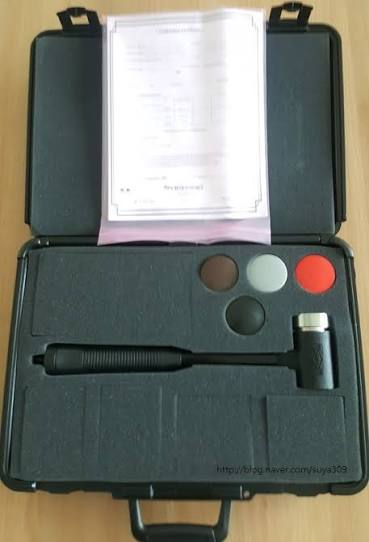
\includegraphics[height=0.13\textheight,keepaspectratio]{figuras/excitacion/martillo_086d20.png}
\end{minipage}
\hfill
\begin{minipage}[c]{0.24\textwidth}
\centering
\textbf{(b) Diseño conceptual del martillete}\par\smallskip
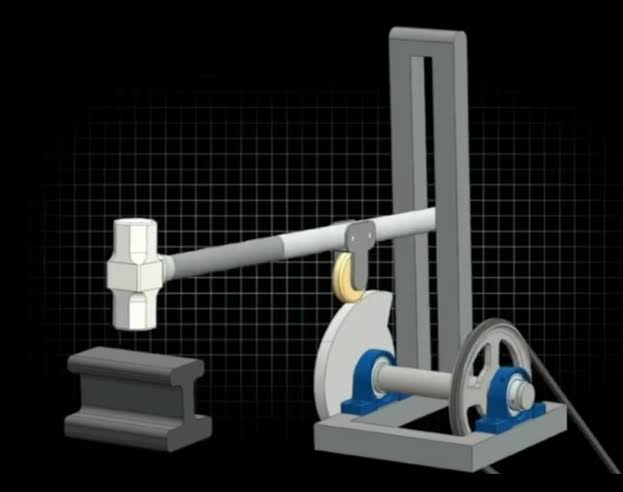
\includegraphics[width=0.94\textwidth]{figuras/excitacion/concepto_martillete_da_vinci.png}
\end{minipage}
\hfill
\begin{minipage}[c]{0.53\textwidth}
\centering
\textbf{(c) Estado actual del prototipo}\par\smallskip
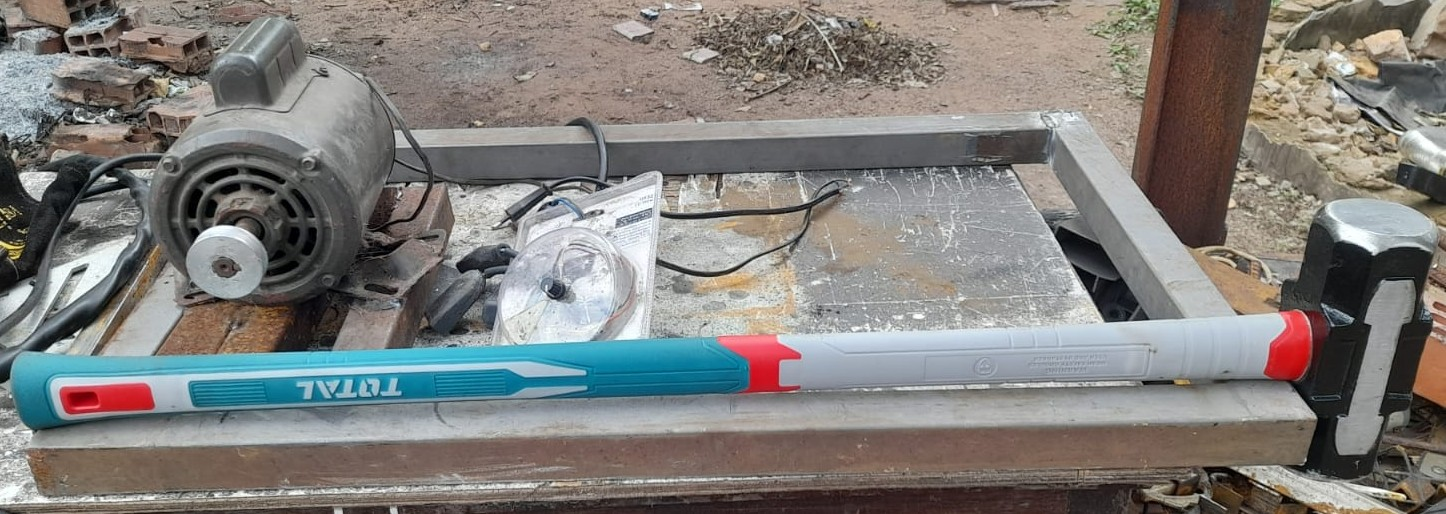
\includegraphics[width=\textwidth]{figuras/excitacion/estado_actual_martillete.jpg}
\end{minipage}

\medskip
\begin{minipage}[c]{0.32\textwidth}
\centering
\textbf{(d) Principio ICP}\par\smallskip
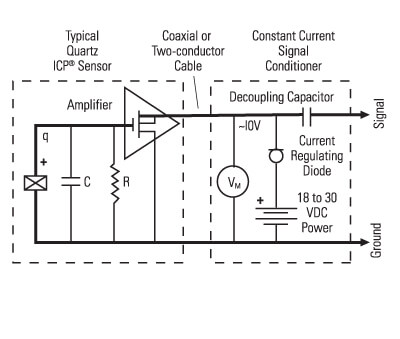
\includegraphics[width=\textwidth]{figuras/excitacion/principio_icp_corriente_constante.png}
\end{minipage}
\hfill
\begin{minipage}[c]{0.64\textwidth}
\centering
\textbf{(e) Acondicionamiento implementado en el PSoC}\par\smallskip
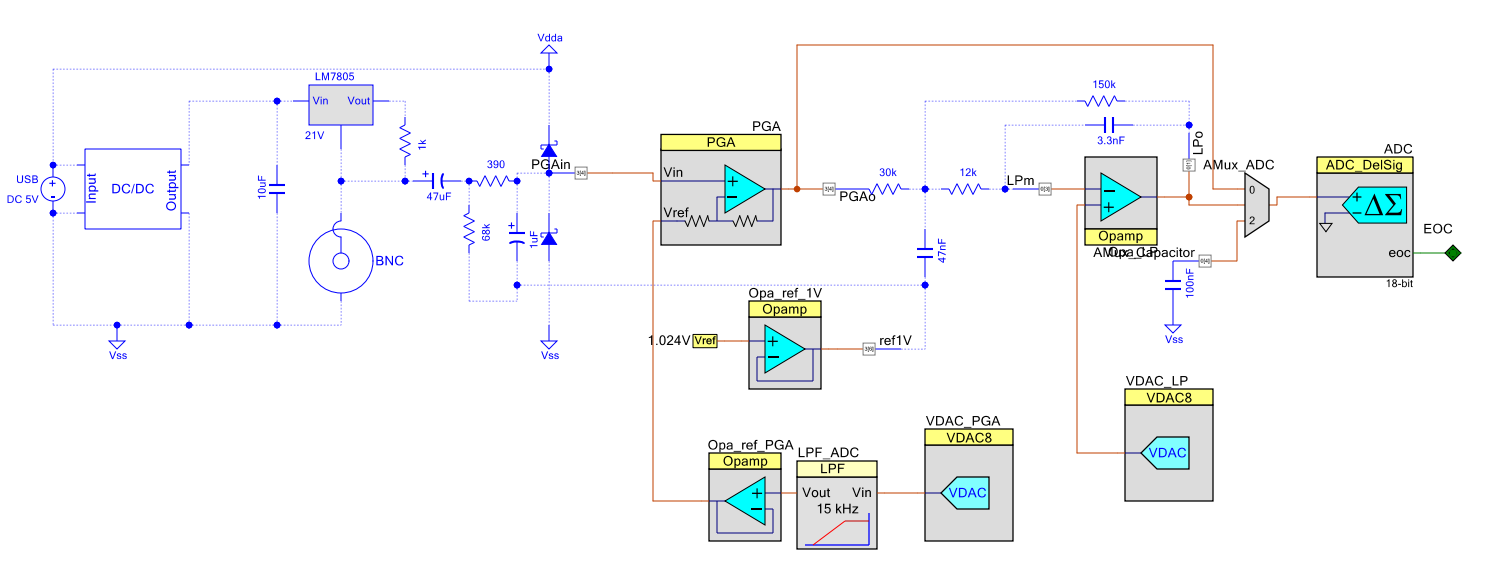
\includegraphics[width=\textwidth]{figuras/excitacion/acondicionamiento_martillo_psoc.png}
\end{minipage}
\caption{Excitación sísmica. (a) Martillo instrumentado utilizado. (b) Diseño
conceptual del martillete. (c) Estado actual: bastidor, motor y martillo antes de
integrar transmisión, guiado y control. (d) Alimentación y desacople ICP recomendados
por PCB. (e) Fuente de corriente con LM7805, acondicionamiento y ADC implementados.}
\label{fig:acondicionamiento-martillo-davinci}
\end{figure*}
\FloatBarrier

\section{Transducción sísmica: alternativas y restricción impuesta por el SM-24}
\label{sec:transductores}

El transductor fija la componente observada, sensibilidad, banda y ruido antes de que
intervenga el amplificador. La electrónica puede amplificar, filtrar o compensar
parcialmente su respuesta, pero no cambia la dinámica mecánica. Esta sección compara las
familias aplicables a Rayleigh y cuantifica el desajuste entre el SM-24 disponible, de
\SI{10}{\hertz}, y la banda requerida para investigar hasta \SI{50}{\meter}.

\subsection{Qué debe preservar el transductor}

Una onda Rayleigh produce movimiento elíptico en el plano vertical; un MASW activo
convencional usa receptores verticales para captar su componente dominante. Los sensores
horizontales o triaxiales son necesarios para Love, elipticidad, HVSR o ciertos arreglos
pasivos, no para una curva Rayleigh básica~\cite{Foti2014,Park1999}.

El registro de un canal puede representarse como

\begin{equation}
\begin{aligned}
    y_j(t)&=h_{s,j}(t)*q_j(t)+n_j(t),\\
    Y_j(f)&=H_{s,j}(f)Q_j(f)+N_j(f),
\end{aligned}
    \label{eq:transductor-medicion}
\end{equation}

donde $q_j$ es desplazamiento, velocidad o aceleración; $H_{s,j}$ incluye sensor y
acoplamiento; y $N_j$ es ruido. MASW usa diferencias de fase: una respuesta idéntica en
todos los canales se cancela, mientras diferencias de amortiguamiento, inclinación o
acoplamiento introducen fase diferencial y sesgan la velocidad aparente.

Para obtener la dispersión importa principalmente que cada frecuencia conserve una
relación de fase coherente entre canales y una relación señal--ruido útil. La variable
física medida es secundaria mientras la respuesta del sensor sea conocida y uniforme
en todo el arreglo.

\subsection{Alternativas y costos de referencia}

La comparación reúne magnitud, banda, ruido, alimentación, ejes y precio del elemento;
no incluye cableado, carcasa, PCB, digitalización, importación ni impuestos. Los precios
se consultaron el 18 de agosto de 2026 y sólo indican órdenes de magnitud.

\begin{table*}[ht]
\centering
\footnotesize
\caption{Alternativas de transducción y costo del elemento sensor.}
\begin{tabularx}{\textwidth}{@{}>{\raggedright\arraybackslash}p{0.15\textwidth} >{\raggedright\arraybackslash}p{0.23\textwidth} >{\raggedright\arraybackslash}p{0.19\textwidth} Y@{}}
\toprule
\textbf{Referencia} & \textbf{Magnitud y banda} & \textbf{Precio publicado} &
\textbf{Evaluación para el arreglo} \\
\midrule
SM-24, \SI{10}{\hertz} & Geófono vertical; velocidad; respuesta plana sobre $f_n$ &
69,95 USD con disco aislante & Pasivo y estándar en MASW; 24 elementos cuestan
aproximadamente 1.679 USD, pero la respuesta cae bajo $f_n$~\cite{SparkFunSM24} \\
RTC, \SI{4.5}{\hertz} & Geófono vertical; velocidad; mayor extensión hacia bajas
frecuencias & 92--154 USD según carcasa & Sustitución directa: 2.208--3.696 USD para 24
puntos~\cite{RTClark45} \\
ADXL355 & Aceleración desde continua; triaxial, ADC de 20 bits & 70,93 USD por unidad;
41,84 USD a 1.000 & Integración simple, pero deben validarse ruido, sincronización y
acoplamiento del nodo completo~\cite{DigiKeyADXL355,AnalogDevicesADXL355} \\
PCB 393B31 & Aceleración, \SIrange{0.1}{200}{\hertz}; $1~\mu g$ RMS & Por cotización &
Muy bajo ruido, pero requiere IEPE de \SIrange{24}{28}{\volt} y adquisición compatible
~\cite{PCB393B31} \\
Güralp 3ESPC & Velocidad triaxial, 60 s--\SI{100}{\hertz} & Por cotización & Cubre bajas
frecuencias con bajo ruido; es un instrumento profesional completo~\cite{Guralp3ESPC} \\
\bottomrule
\end{tabularx}
\end{table*}

Los geófonos siguen siendo la opción natural para MASW activo por sensibilidad,
robustez y pasividad. Reducir $f_n$ conserva mejor las longitudes de onda grandes, pero
aumenta el costo. Un MEMS tampoco es automáticamente más económico: en el ADXL355 la
densidad de ruido especificada es $22{,}5~\mu g/\sqrt{\mathrm{Hz}}$, y el costo real
depende además de encapsulado, calibración y comunicación~\cite{AnalogDevicesADXL355}.

\subsection{SM-24: restricción de partida}

El SM-24 de \SI{10}{\hertz} se empleó porque estaba disponible en la Facultad, no porque
resultara de optimizar la profundidad. Su $f_n$ dificulta recuperar los pocos hertz
asociados a \SI{50}{\meter}; aun así, es vertical, pasivo, robusto, documentado y de
costo compatible con un arreglo académico. Su salida analógica permite además estudiar
el acondicionamiento como parte central del proyecto.

\begin{figure}[!ht]
\centering
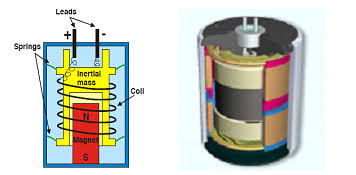
\includegraphics[width=\columnwidth]{sm24_esquema_interno.png}\par\smallskip
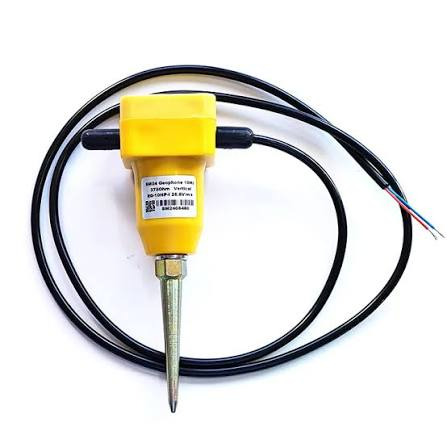
\includegraphics[width=0.80\columnwidth]{sm24_fotografia_cableado.png}
\caption{Principio constructivo de un geófono electromagnético y SM-24 encapsulado
con cable y punta de acoplamiento al terreno.}
\label{fig:sm24-fisico-respuesta}
\end{figure}

Sus parámetros nominales principales son~\cite{SM24}:

\begin{table}[!ht]
\centering
\scriptsize
\caption{Parámetros nominales del SM-24.}
\begin{tabularx}{\columnwidth}{@{}Y>{\raggedleft\arraybackslash}p{0.36\columnwidth}@{}}
\toprule
\textbf{Parámetro} & \textbf{Valor} \\
\midrule
Frecuencia natural & \SI{10}{\hertz} $\pm2{,}5\%$ \\
Sensibilidad & \SI{28.8}{\volt\second\per\meter} $\pm2{,}5\%$ \\
Amortiguamiento abierto & $\zeta=0{,}25$ \\
Amortiguamiento con \SI{1339}{\ohm} & $\zeta=0{,}60$ \\
Resistencia de bobina & \SI{375}{\ohm} $\pm2{,}5\%$ \\
Masa móvil & \SI{11}{\gram} \\
Frecuencia espuria típica & $>\SI{240}{\hertz}$ \\
\bottomrule
\end{tabularx}
\end{table}

\subsection{Modelo dinámico del SM-24: velocidad y aceleración}

Sea $x_g$ el desplazamiento de la carcasa unida al suelo, $x_m$ el de la masa móvil y
$z=x_m-x_g$ el desplazamiento relativo. El sistema masa--resorte--amortiguador satisface

\begin{equation}
\begin{aligned}
    m\ddot z+c\dot z+kz&=-m\ddot x_g,\\
    \omega_n&=\sqrt{\frac{k}{m}},
    &\zeta&=\frac{c}{2\sqrt{km}}.
\end{aligned}
    \label{eq:sm24-mecanico}
\end{equation}

La bobina genera una fuerza electromotriz proporcional a la velocidad relativa:

\begin{equation}
    v_o(t)=G_0\dot z(t),
\end{equation}

por lo que, tomando como entrada la velocidad del suelo,

\begin{equation}
    H_v(s)=\frac{V_o(s)}{\dot X_g(s)}
    =-G_0\frac{s^2}{s^2+2\zeta\omega_ns+\omega_n^2}.
    \label{eq:sm24-velocidad}
\end{equation}

Con $r=\omega/\omega_n$, la magnitud normalizada es

\begin{equation}
    \frac{|H_v(j\omega)|}{G_0}
    =\frac{r^2}{\sqrt{(1-r^2)^2+(2\zeta r)^2}}.
    \label{eq:sm24-magnitud}
\end{equation}

La aceleración del suelo es $A_g(s)=s^2X_g(s)=s\dot X_g(s)$. Por tanto, la misma salida
del SM-24 puede expresarse respecto de la aceleración como

\begin{equation}
    H_a(s)=\frac{V_o(s)}{A_g(s)}
    =\frac{H_v(s)}{s}
    =-G_0\frac{s}{s^2+2\zeta\omega_ns+\omega_n^2}.
    \label{eq:sm24-aceleracion}
\end{equation}

Su magnitud, normalizada por $G_0/\omega_n$, es

\begin{equation}
    \frac{\omega_n|H_a(j\omega)|}{G_0}
    =\frac{r}{\sqrt{(1-r^2)^2+(2\zeta r)^2}}.
    \label{eq:sm24-magnitud-aceleracion}
\end{equation}

El geófono sin compensar se usa habitualmente referido a velocidad porque
$H_v\rightarrow-G_0$ por encima de $f_n$: allí su respuesta es aproximadamente plana.
Referido a aceleración, $H_a$ es pasabanda y no presenta una meseta con el
amortiguamiento nominal.

Por debajo de $f_n$, $|H_v|$ cae como $r^2$ (\SI{40}{\decibel\per decade}) y $|H_a|$
como $r$ (\SI{20}{\decibel\per decade}); son dos referencias de una misma tensión de
salida, no dos modos de funcionamiento distintos.

\begin{figure}[!ht]
\centering
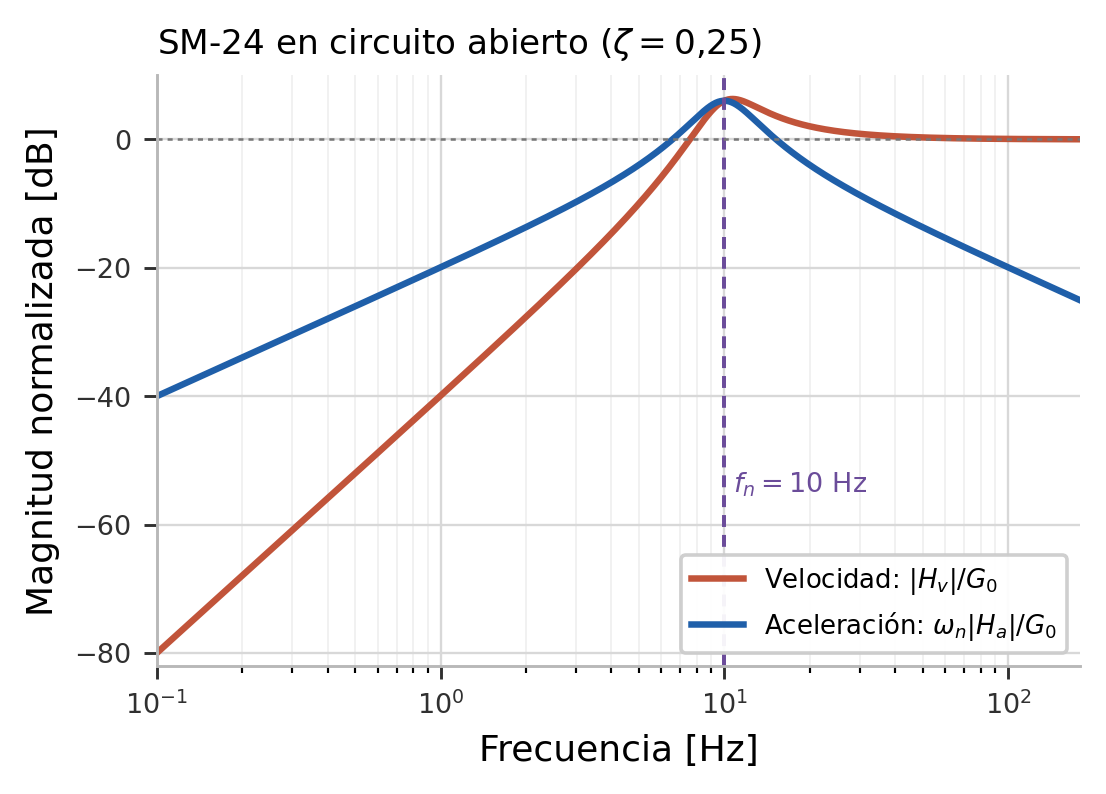
\includegraphics[width=\columnwidth]{respuesta_sm24_vel_acel.png}
\caption{Modelo nominal del SM-24 en circuito abierto. Ambas referencias se muestran
en los mismos ejes: bajo $f_n$ caen \SI{40}{\decibel\per decade} y
\SI{20}{\decibel\per decade}; sobre $f_n$, la referencia a velocidad se aplana y la
referencia a aceleración cae \SI{20}{\decibel\per decade}.}
\label{fig:sm24-modelo}
\end{figure}

\subsection{La banda exigida por el objetivo de profundidad}

La propuesta original planteó caracterizar hasta \SI{50}{\meter}. Como estimación de
diseño se usa

\begin{equation}
    \lambda_R=\frac{c_R}{f}.
\end{equation}

Longitudes de \SIrange{100}{150}{\meter} y velocidades Rayleigh de
\SIrange{150}{500}{\meter\per\second} sitúan la información profunda en
\SIrange{1}{5}{\hertz}. No es una conversión universal profundidad--frecuencia, sino una
comparación preliminar con la respuesta del sensor.

El conflicto queda cuantificado al evaluar la ecuación~\eqref{eq:sm24-magnitud}:

\begin{table}[!ht]
\centering
\scriptsize
\caption{Respuesta nominal del SM-24 en circuito abierto, normalizada respecto de
velocidad y aceleración.}
\begin{tabular}{@{}rrrr@{}}
\toprule
$f$ & $f/f_n$ & $|H_v|/G_0$ & $\omega_n|H_a|/G_0$ \\
\midrule
\SI{1}{\hertz}  & 0,10 & $-40{,}0$ dB & $-19{,}9$ dB \\
\SI{2}{\hertz}  & 0,20 & $-27{,}6$ dB & $-13{,}7$ dB \\
\SI{5}{\hertz}  & 0,50 & $-10{,}0$ dB & $-4{,}0$ dB \\
\SI{10}{\hertz} & 1,00 & $+6{,}0$ dB & $+6{,}0$ dB \\
\SI{20}{\hertz} & 2,00 & $+2{,}0$ dB & $-4{,}0$ dB \\
\bottomrule
\end{tabular}
\end{table}

En la referencia a velocidad, la salida cae \SI{27.6}{\decibel} a \SI{2}{\hertz} y
\SI{40}{\decibel} a \SI{1}{\hertz}; normalizada respecto de aceleración, cae
\SI{13.7}{\decibel} y \SI{19.9}{\decibel}. La diferencia refleja pendientes de
\SI{40}{\decibel\per decade} y \SI{20}{\decibel\per decade}; no crea señal adicional
en los terminales.

\subsection{Implicación para el acondicionamiento}

La tesis asume el desajuste del SM-24 como problema de instrumentación: determinar cuánto
contenido de baja frecuencia puede conservarse mediante una cadena analógica de bajo
ruido que compense la región atenuada y preserve fase y rango dinámico. No se considera
al SM-24 óptimo ni se atribuye a la electrónica la capacidad de eliminar su límite
mecánico. La siguiente sección desarrolla esa estrategia.

\section{Acondicionamiento, instrumentación y digitalización}
\label{sec:acondicionamiento-digitalizacion}

El frente analógico debe convertir una tensión diferencial pequeña en una secuencia que
aproveche el ADC, preserve la fase y se adquiera de forma determinista; la transmisión
se trata después.

Si $v_d(t)$ es la tensión diferencial de entrada,

\begin{equation}
\begin{aligned}
v_{\mathrm{ADC}}(t)={}&V_{\mathrm{CM}}+\left[h_{\mathrm{AFE}}(t)*v_d(t)\right]\\
&+v_{\mathrm{os}}(t)+n_{\mathrm{AFE}}(t),\\
x[n]={}&Q_{B,V_{\mathrm{span}}}\!\left\{v_{\mathrm{ADC}}(nT_s)\right\}.
\end{aligned}
\label{eq:afe-general}
\end{equation}

La ecuación reúne rechazo de modo común, ganancia programable, conformación espectral,
control del punto de operación, digitalización conocida y transferencia determinista a
memoria. El \emph{offset} acumulado puede agotar el rango aun sin señal.

\subsection{Compensador de polos desacoplados}

Tras evaluar varias arquitecturas se adoptó la forma $1-\mathrm{BP}$ propuesta e
implementada en \cite{Ma2023}. En ese trabajo, un pasa-banda Sallen--Key y un
amplificador diferencial restan la rama BP del camino directo.

La caída de \SI{27.7}{\decibel} a \SI{2}{\hertz} exige compensación antes del ADC si se
quiere observar contenido próximo a \SI{1}{\hertz}. Ma et al. muestran que conservar
$f_n$ y elevar el amortiguamiento efectivo extiende la respuesta aproximadamente plana a
aceleración entre

\begin{equation}
f_1\simeq\frac{f_n}{2\zeta_1},
\qquad
f_2\simeq2\zeta_1f_n.
\end{equation}

Por tanto, $\zeta_1$ se elige para llevar $f_1$ hasta la zona de interés. El valor de
$f_2$ no es un objetivo porque la aplicación no requiere extender la banda superior;
sólo debe conservarse la simetría logarítmica $f_1f_2=f_n^2$ alrededor de $f_n$.

Como los quiebres quedan muy separados, el $Q$ requerido es bajo: Sallen--Key o MFB no
aportan en este régimen y distribuyen cada polo entre más componentes, una desventaja
frente a tolerancias y valores disponibles.

Se desacoplaron los polos: uno en la entrada ($R_1$ serie $C_1$) y otro en la
realimentación ($R_2$ paralelo $C_2$) de un inversor. Cada uno depende de un solo par
$RC$. La inversión se reutiliza para combinar las ramas con un sumador inversor, sin
pareamiento, y su realimentación aporta el primer polo pasa-bajos.

\subsection{Ajuste y selección de componentes}

La cancelación depende de la proporción entre la rama directa y BP. Un potenciómetro en
serie con BP permite corregir esa proporción en cada unidad.

La red resultante se diseñó a partir del modelo dinámico del geófono,

\begin{equation}
H_{\mathrm{geo}}(s)=\frac{\omega_n s}
{s^2+2\zeta_0\omega_n s+\omega_n^2},
\end{equation}

donde $\zeta_0$ es el amortiguamiento nominal del SM-24. Se busca que la cadena formada
por el compensador y el geófono presente el amortiguamiento $\zeta_1$ requerido para
llevar el quiebre inferior a la zona de interés. Entonces

\begin{equation}
H_{\mathrm{comp}}(s)=
\frac{s^2+2\zeta_0\omega_n s+\omega_n^2}{s^2+2\zeta_1\omega_n s+\omega_n^2},
\end{equation}

y separar el término constante da la forma que se implementa en el circuito, un camino
directo menos un pasa-banda:

\begin{equation}
H_{\mathrm{comp}}(s)=1-\frac{2(\zeta_1-\zeta_0)\omega_n s}
{s^2+2\zeta_1\omega_n s+\omega_n^2}.
\label{eq:comp-afe}
\end{equation}

Se relevaron los pasivos disponibles y se incluyó el modelo no ideal del operacional del
PSoC: ganancia de continua de
\SI{90}{\decibel}, producto ganancia--ancho de banda de \SI{8}{\mega\hertz}, impedancia
de entrada de \SI{35}{\mega\ohm} y resistencia de salida de \SI{10}{\ohm}. Con ese modelo
se resolvió una búsqueda por evolución diferencial sobre la malla de valores comerciales
para minimizar el error respecto de la Ec.~\eqref{eq:comp-afe}. La búsqueda admitió
capacitores en paralelo.

Los quiebres necesarios para aproximar la banda buscada producen un amortiguamiento
efectivo muy alto: con los valores poblados se obtiene $f_0=\SI{10.21}{\hertz}$ y
$\zeta_1\simeq938$. En la zona central, el modelo compensado queda escalado por
$1/(2\zeta_1)\simeq5.3\times10^{-4}$, una atenuación de 1876 veces. La ganancia
se repartió para recuperar ese nivel sin concentrar todo el margen en un solo bloque:
la entrada instrumental
aporta $\times2$, el PGA es ajustable entre $\times1$ y $\times50$, el sumador aporta
$\times3.6$ y el pasa-bajos $\times5$. A máxima ganancia el producto es $\times1800$,
por lo que la señal del geófono llega al ADC con aproximadamente el \SI{96}{\percent}
de su escala previa a la compensación.

Como comprobación inicial se barrió la electrónica entre la salida monitoreada del PGA
y la entrada del ADC. La respuesta medida se encadenó en frecuencia con el modelo
nominal del SM-24 referido a aceleración para estimar la forma de la cadena completa.
En la realimentación del sumador se incorporó el polo real
$p_1=-2\pi(393)\,\mathrm{rad/s}$. La sección MFB se dimensionó con
$f_a=\SI{300}{\hertz}$ y $\zeta_a=0.691$; de
$p=-\zeta_a\omega_a\pm j\omega_a\sqrt{1-\zeta_a^2}$ resultan
$p_{2,3}\simeq2\pi(-207\pm j217)\,\mathrm{rad/s}$. El polo del sumador y este par
conjugado forman el antialias Bessel de tercer orden, elegido por su fase
aproximadamente lineal.

Las ganancias se mantuvieron conservadoras porque, al aumentarlas, cada paso del VDAC
también se amplifica: la calibración pierde resolución y la deriva, especialmente en el
sumador, se vuelve difícil de controlar. Como revisión pendiente se agregó una etapa
PGA de salida ajustable hasta $\times50$ y se sustituyeron las cuatro referencias VDAC
de \SIrange{0}{4.08}{\volt} por IDAC usados como DAC de tensión. Con la resistencia de
conversión propuesta, el ajuste se concentra aproximadamente entre
\SIrange{2.06}{3.02}{\volt}, en lugar de desperdiciar códigos fuera de la región útil.
La arquitectura permitiría otros $\times50$ de ganancia, pero aún requiere pruebas en
placa.

\begin{figure*}[p]
\centering
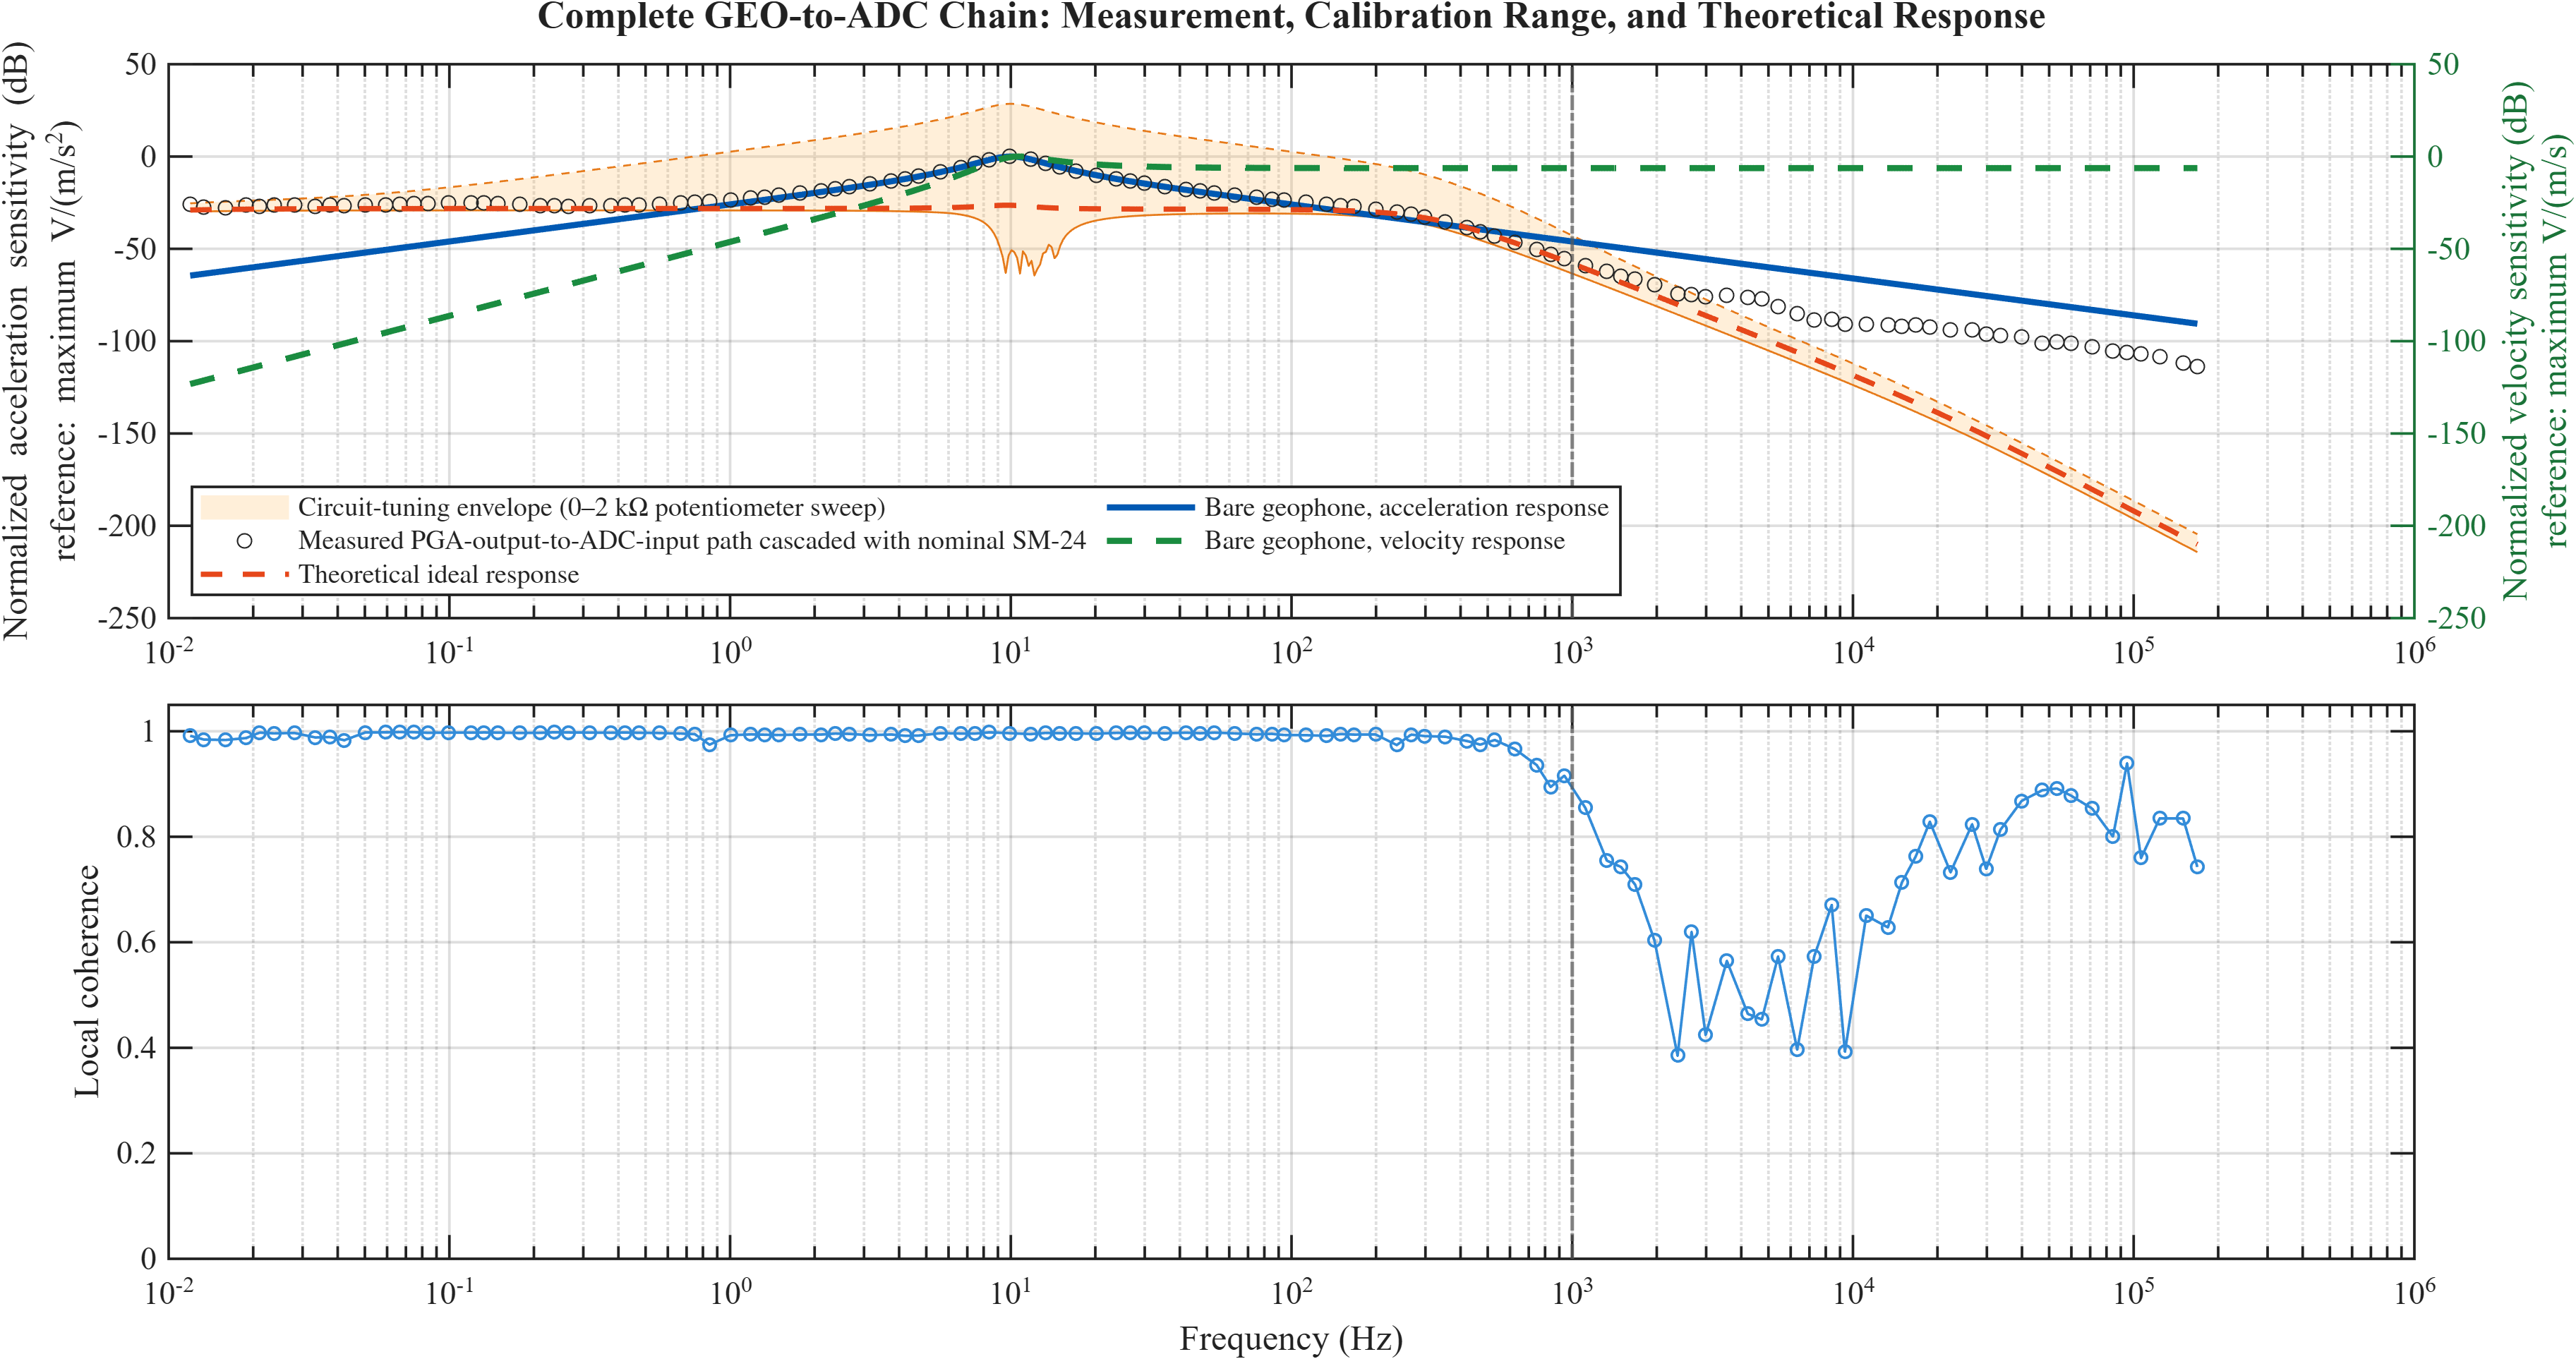
\includegraphics[width=0.97\textwidth,height=0.285\textheight,keepaspectratio]
{respuesta_geofono_afe_medida.png}
\caption{Cadena geófono--ADC: respuesta electrónica medida encadenada con el SM-24,
margen de ajuste y coherencia del barrido. La pérdida de coherencia próxima a
\SI{1}{\kilo\hertz} limita la interpretación superior; es una verificación de forma,
no una medición sísmica calibrada extremo a extremo.}
\label{fig:respuesta-geofono-afe}

\vspace{0.25em}
\textbf{(a) Ruta analógica empleada}\par
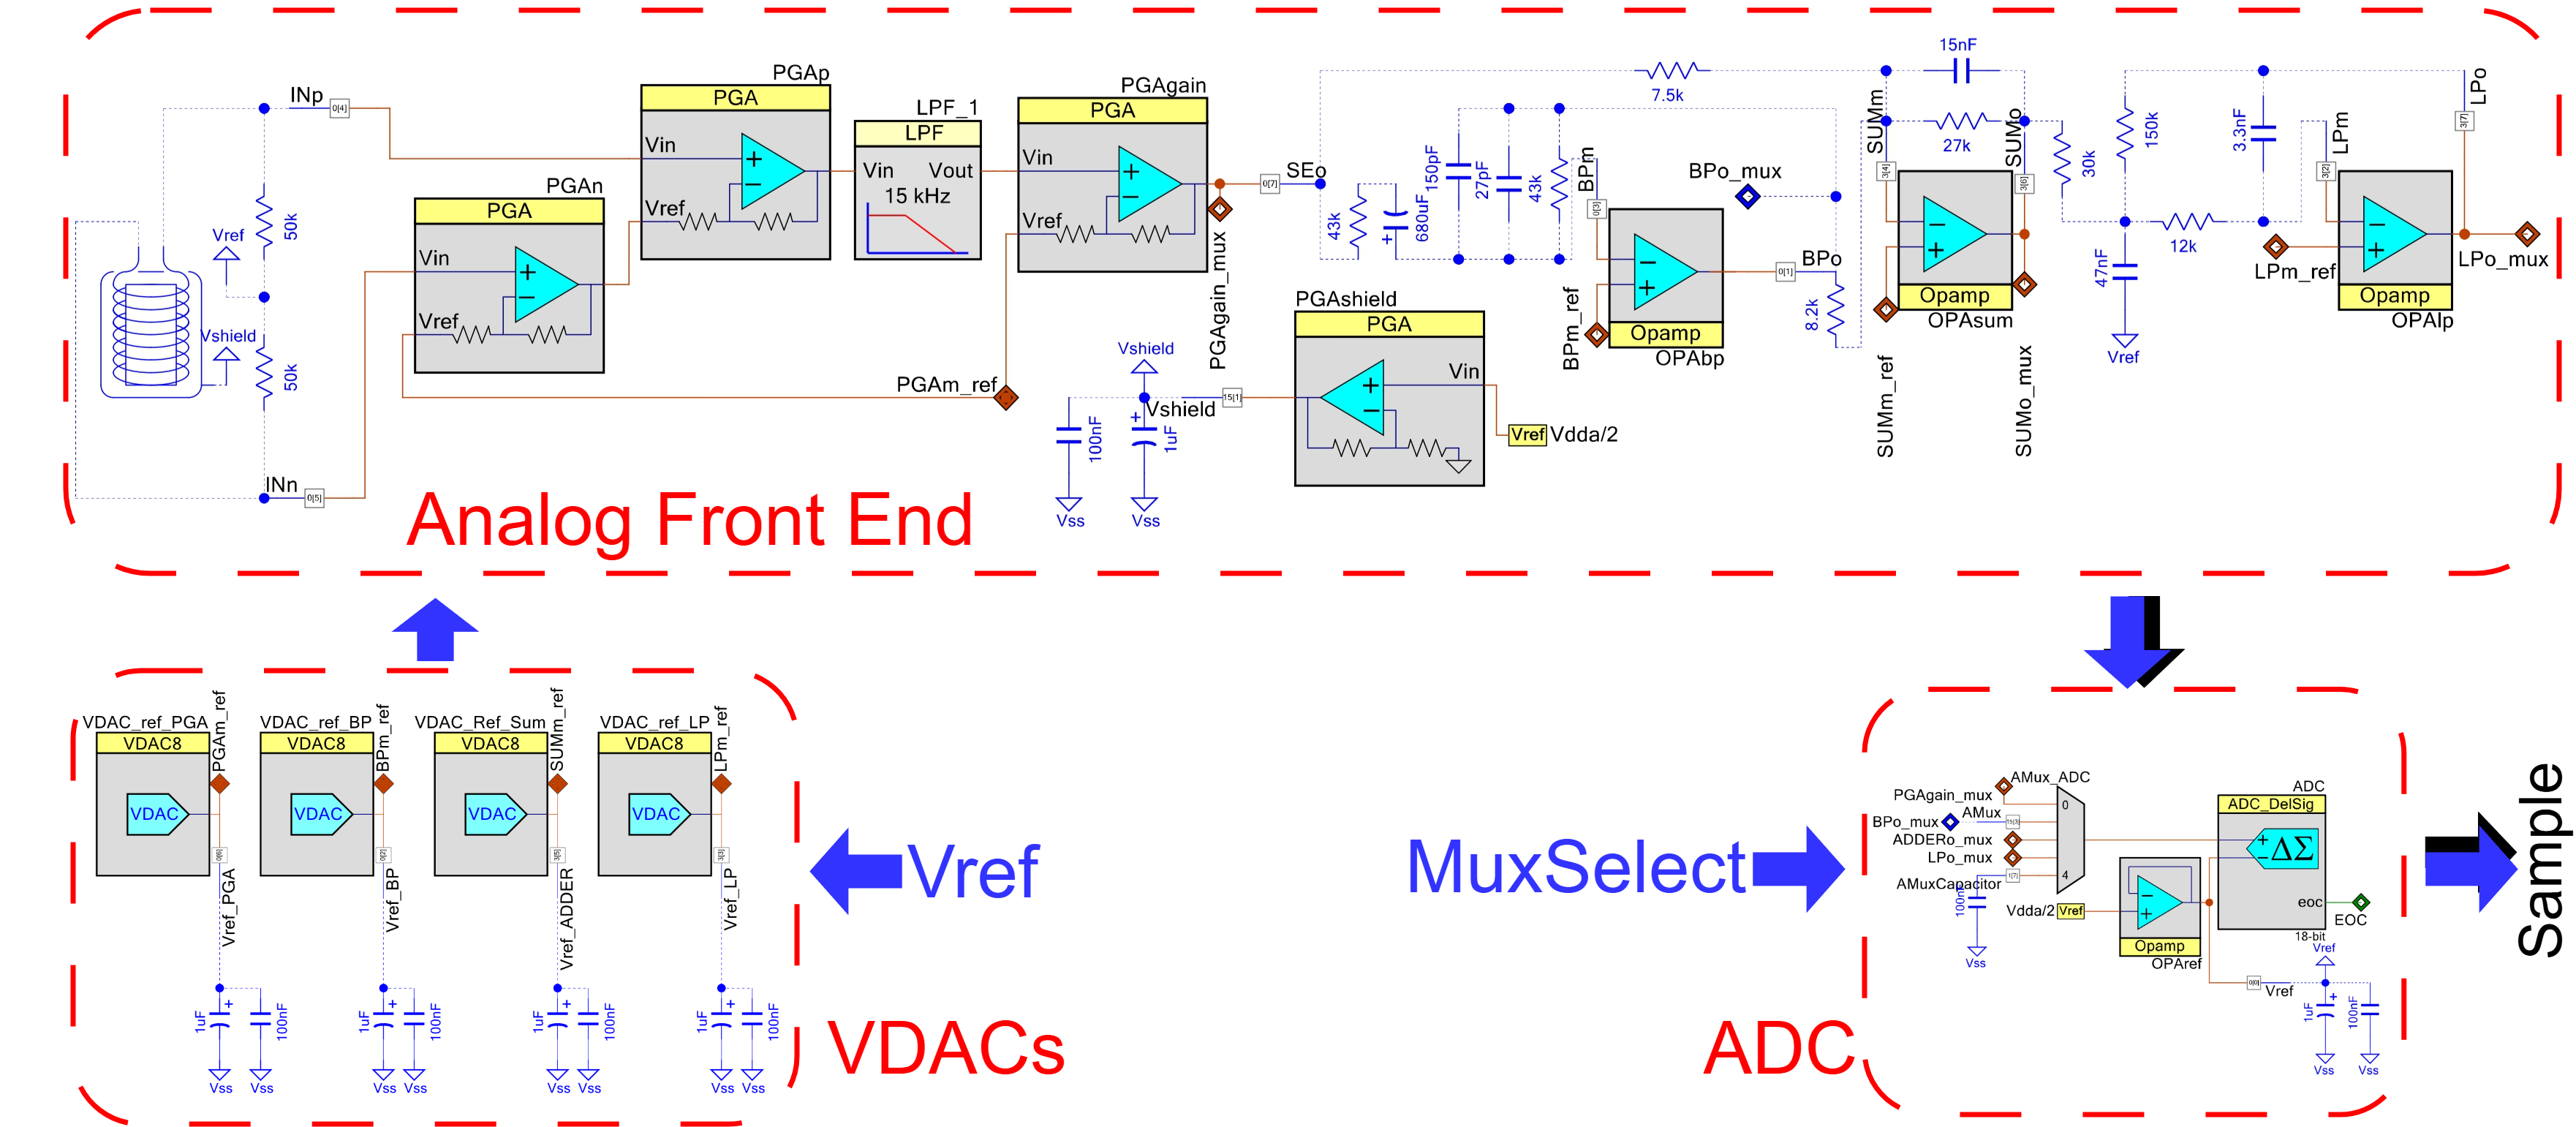
\includegraphics[width=0.99\textwidth,height=0.255\textheight,keepaspectratio]
{arquitectura_analogica_psoc.png}\par
\textbf{(b) Arquitectura digital}\par
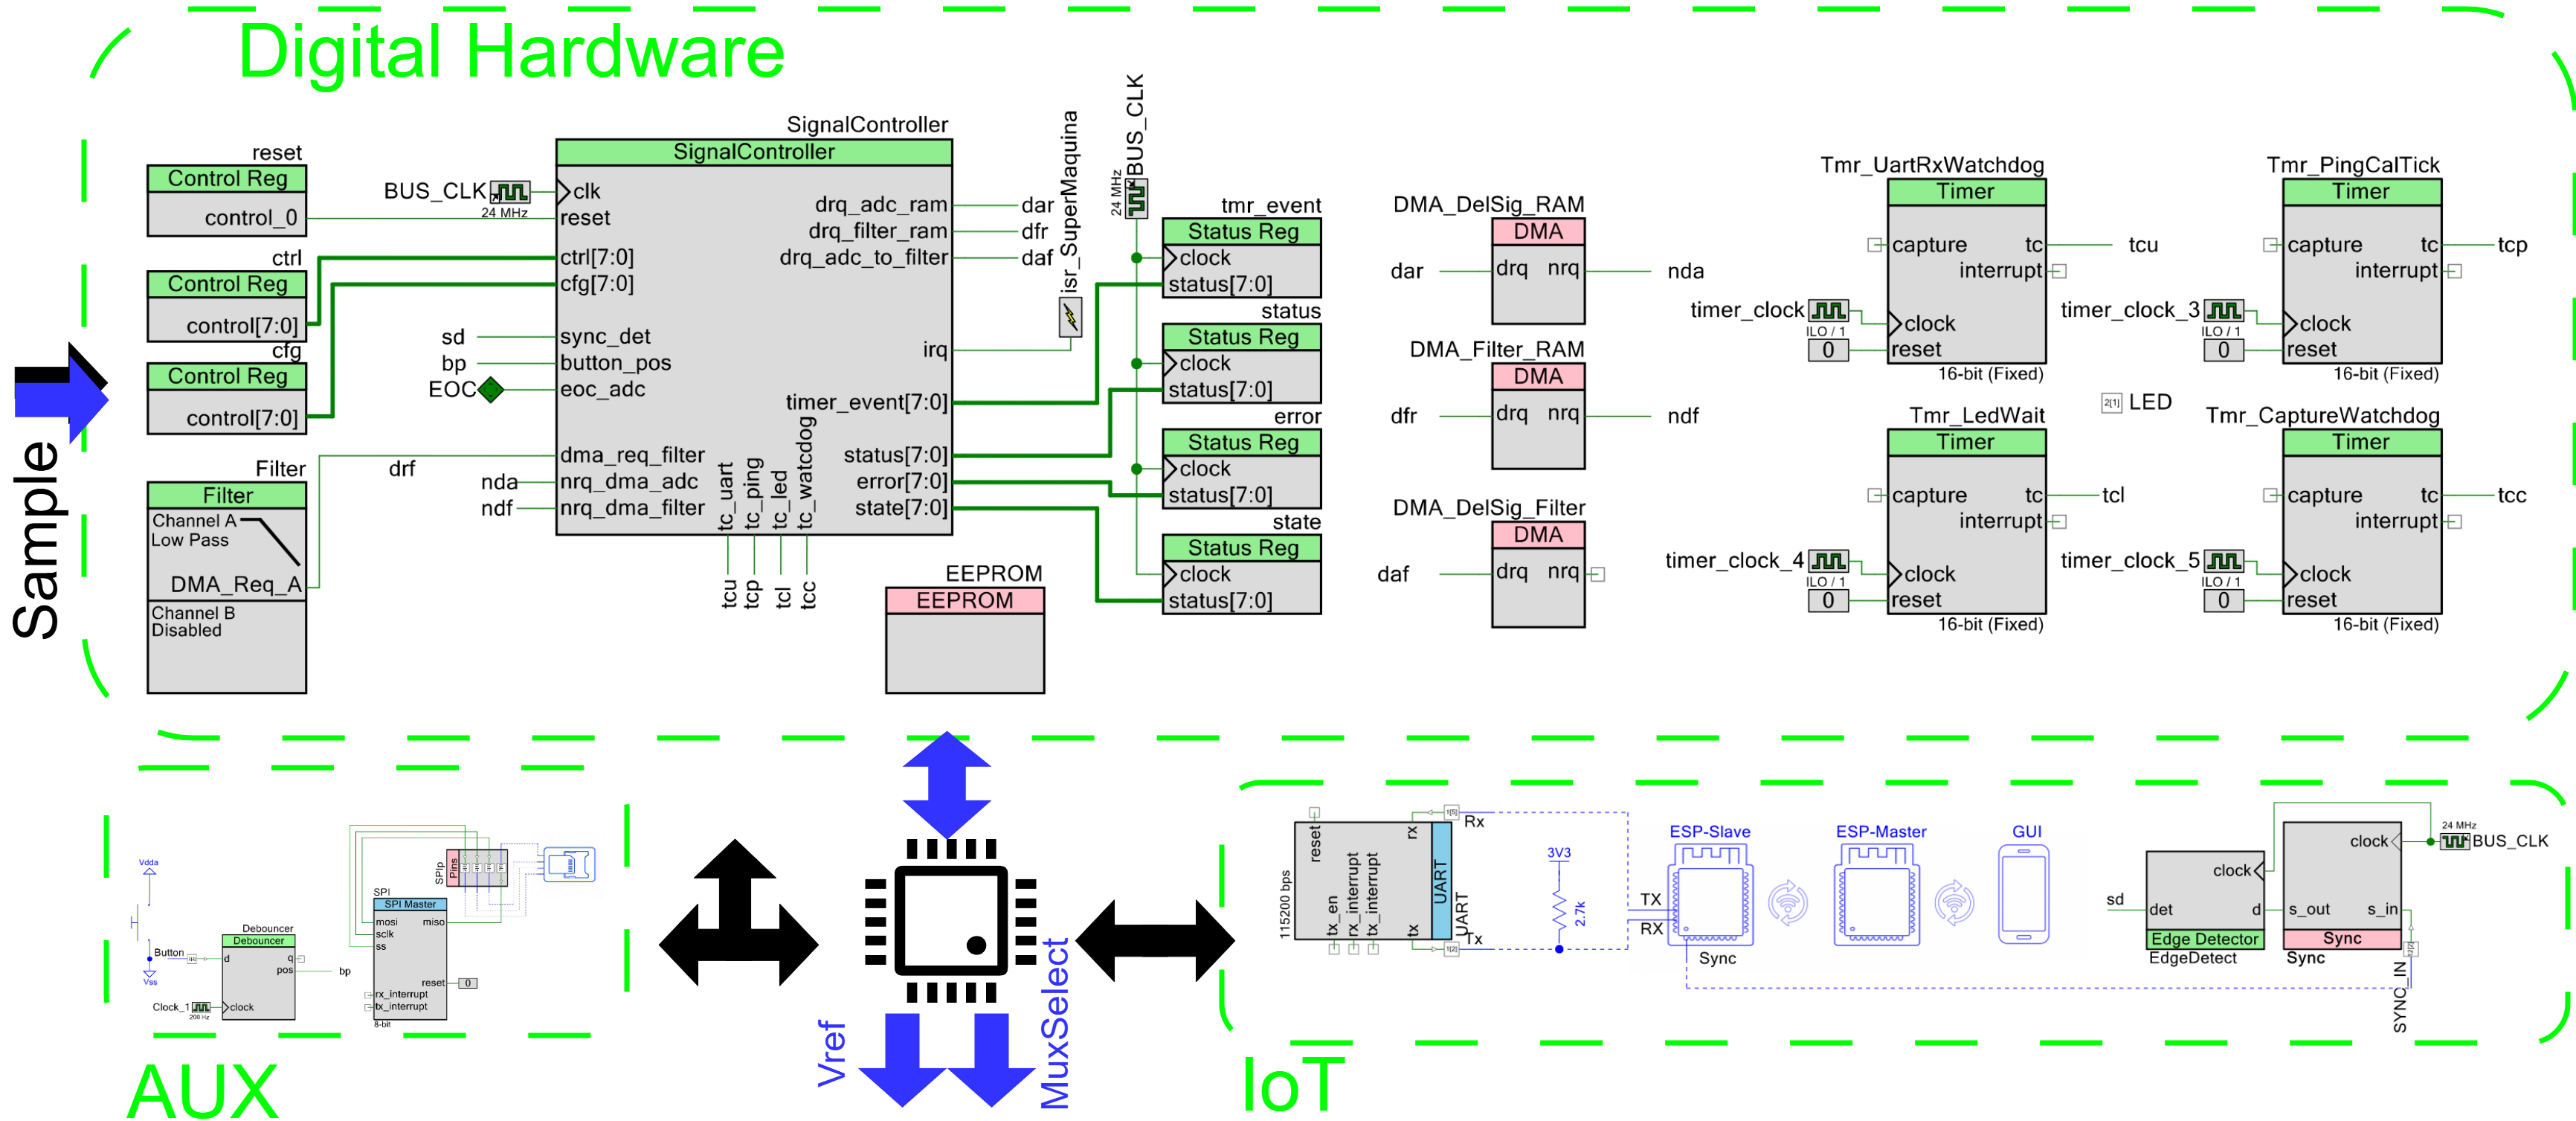
\includegraphics[width=0.99\textwidth,height=0.255\textheight,keepaspectratio]
{arquitectura_digital_psoc.png}
\caption{Arquitectura utilizada en las mediciones: acondicionamiento, referencias,
AMux y ADC $\Delta\Sigma$; captura, filtrado, DMA, memoria y temporización.}
\label{fig:topdesign-analogico}
\end{figure*}

\begin{figure*}[!t]
\centering
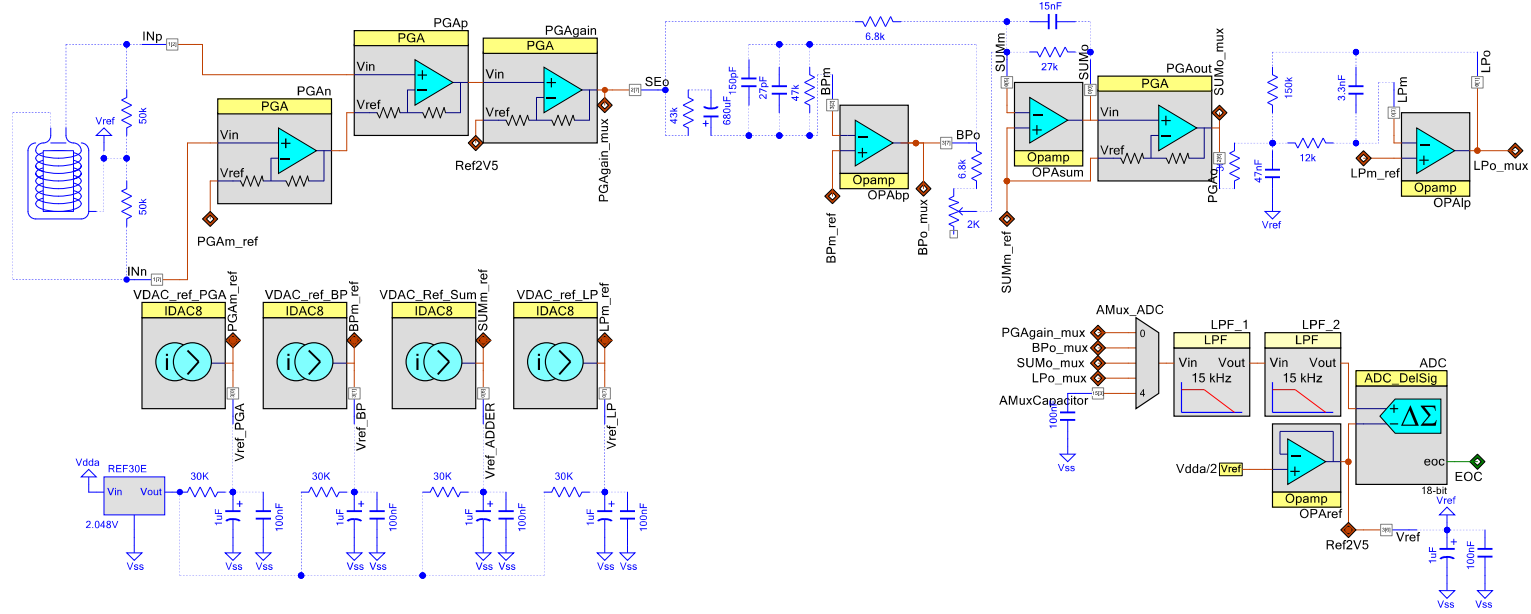
\includegraphics[width=0.99\textwidth,height=0.29\textheight,keepaspectratio]
{propuesta_idac_pgaout_nueva.png}
\caption{Nueva propuesta para el frente GEO: PGA de salida y cuatro IDAC concentrados
en la región útil de ajuste. Aporta hasta $\times50$ adicionales y aún no fue empleada
en las mediciones.}
\label{fig:propuesta-idac-pgaout}
\end{figure*}

\subsection{Acople DC y calibración}

Al extender la compensación hacia \SI{1}{\hertz}, el \emph{offset} y la deriva térmica,
en especial del sumador, consumieron el margen del ADC aun sin señal.

Un multiplexor observa cada nodo con el mismo ADC y cada etapa posee referencia
programable. La calibración \emph{foreground} recorre PGA, BP, sumador y pasa-bajos; un
FIR de 128 taps estima el residuo y un PI con banda muerta, saturación y
\emph{anti-windup} corrige la referencia. El orden evita propagar el residuo aguas abajo.
Los códigos se guardan en EEPROM por ganancia, con CRC. Durante la captura el lazo se
desactiva y los códigos quedan fijos.

\subsection{Digitalización y memoria}

El ADC $\Delta\Sigma$ del PSoC~5LP entrega 18 bits nominales a
$F_{s,0}=\SI{2604}{SPS}$ y cuatro rangos bipolares entre $\pm\SI{0.512}{\volt}$ y
$\pm\SI{2.5}{\volt}$. PGA y rango se eligen juntos para usar el menor rango sin saturar.
El DFB filtra por FIR; dos DMA trasladan crudo y filtrado a RAM; y
un bloque de control implementado en Verilog/UDB coordina inicio, ADC, conteo y fin.
El software queda para calibración, persistencia y comandos.

\subsection{Estado de verificación}

Queda medir magnitud y fase extremo a extremo para cada ganancia y rango, ruido referido
a entrada y bits efectivos, dispersión entre placas, deriva térmica y repetibilidad de
la calibración tras migrar las referencias VDAC a IDAC.

\begin{figure}[!tb]
\centering
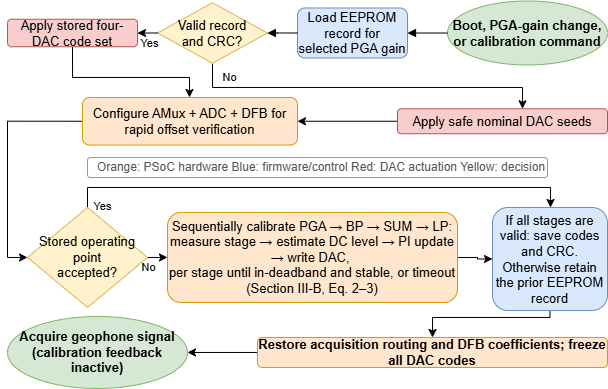
\includegraphics[width=\columnwidth,keepaspectratio]
{flujo_calibracion_horizontal_usuario.png}
\caption{Máquina de estados de la calibración \emph{foreground}: valida los códigos,
ajusta PGA, BP, sumador y pasa-bajos, y restaura la adquisición con códigos fijos.}
\label{fig:maquina-estados-calibracion}
\end{figure}

\section{Transmisión, ingesta e interfaces}
\label{sec:transmision-interfaces}

Una vez acondicionada y digitalizada, la señal debe abandonar cada nodo, llegar sin
ambigüedades a un punto común, conservar su contexto de adquisición y quedar disponible
para revisión y procesamiento:

\begin{equation}
\text{nodos de medida}
\longrightarrow
\text{maestro de campo}
\longrightarrow
\text{servidor de ingesta}
\longrightarrow
\text{revisión y MASW}.
\end{equation}

La primera interfaz controla la adquisición (armar nodos, ajustar parámetros, iniciar o
detener una captura, observar el enlace, exportar); la segunda controla el conjunto de
datos (validar, filtrar, agrupar, alinear, promediar, invertir). Esta separación evita
que el microcontrolador ejecute tareas pesadas y permite seguir trabajando en campo sin
conexión a Internet.

\subsection{Plataforma de comunicación}

Se eligió la familia ESP32 por accesibilidad local, bajo costo, documentación abundante
e integración de Wi-Fi; no se lo usa como instrumento de medida, sino después de la
digitalización: el nodo esclavo empaqueta los datos del frente analógico y los entrega
al maestro. El enlace entre nodos usa ESP-NOW, que da una red directa de baja sobrecarga
sin depender de un \emph{router} en el sitio, a cambio de carga útil limitada por
paquete y entrega no confiable por sí sola; el diseño compensa esto con fragmentación,
numeración de mensajes, confirmaciones, reintentos y almacenamiento local previo a la
subida. El maestro concentra los enlaces ESP-NOW y expone además una red Wi-Fi propia
con una interfaz web embebida accesible desde cualquier teléfono o computadora sin
instalar software; cuando hay conectividad disponible pasa a una fase de enlace,
se asocia a una red externa y transfiere la cola de capturas pendientes.

\subsection{Por qué se desarrollaron varias interfaces}

Cada interfaz resolvió una pregunta de una etapa distinta y dejó funciones que se
trasladaron a la siguiente versión. Se empezó por un osciloscopio MATLAB de un solo
canal para fijar las variables que debían quedar controladas (puerto, referencia DC,
ganancia, filtro) antes de comparar capturas; al incorporar varios nodos, una segunda
aplicación MATLAB agregó una vista de estado global y una pestaña por esclavo, tratando
ya la adquisición como un sistema y no como un canal aislado. Una versión de escritorio
en PyQt reorganizó esto en una herramienta multi-nodo con temas claro/oscuro, útil tanto
en laboratorio como a la intemperie. El paso siguiente fue eliminar la dependencia de
una computadora con MATLAB o Python instalado: la interfaz se embebió como una \emph{SPA}
servida directamente por el maestro, operable desde cualquier navegador y funcional sin
conexión a Internet, con menús de Captura, Esclavos, Preservados, Enlace y Log. En
paralelo se prototipó en PyQt, y luego en un servidor web, el flujo de posprocesado
completo (filtros, agrupamiento, enfase, promedios, \emph{waterfall}, dispersión e
inversión MASW), migrando finalmente a un servidor FastAPI para tener una dirección
conocida, estado persistente entre campañas y acceso remoto sin reinstalar nada en cada
equipo de campo.

\begin{table}[ht]
\centering
\small
\begin{tabularx}{\textwidth}{@{}p{0.20\textwidth}p{0.23\textwidth}Y@{}}
\toprule
\textbf{Interfaz} & \textbf{Uso principal} & \textbf{Aporte al diseño} \\
\midrule
MATLAB: alcance USB & Verificar el canal individual & Visualización cruda, referencia DC, FIR, guardado de muestras. \\
MATLAB: InterfaceESP & Probar maestro y esclavos & Sincronización, lotes, control de PGA/FIR por nodo, depuración. \\
PyQt: adquisición & Operar varios nodos & Escritorio multipestaña, estado de enlace, gráficos simultáneos. \\
SPA embebida & Operar en campo sin instalar software & Control desde el navegador, funcionamiento fuera de línea. \\
PyQt: revisión & Explorar el flujo científico & Filtros, grupos, enfase, promedios, \emph{waterfall} y MASW. \\
Servidor FastAPI & Ingestar y procesar en una dirección conocida & Acceso remoto, estado persistente entre campañas. \\
\bottomrule
\end{tabularx}
\caption{Funciones y alcance de las interfaces desarrolladas.}
\label{tab:evolucion-interfaces}
\end{table}

\begin{figure}[ht]
\centering

\includegraphics[width=0.8\textwidth,height=0.62\textheight,keepaspectratio]{esp_historico/07_pga_pgaout/01_captura_completa.png}
\caption{Estado vigente de la SPA embebida: cinco menús (Captura, Esclavos,
Preservados, Enlace, Log), decimación, límites de RAM/SD, selección PGA/PGAout y
subida al servidor. Frente a la primera versión ejecutable, la interfaz pasó de
exponer sólo transporte a exponer una operación de campo completa.}
\label{fig:spa-hito7-resumen}
\end{figure}

\subsection{Resultados reproducibles: estado actual y límites}

Además de las interfaces, el repositorio conserva salidas numéricas generadas por los
scripts de análisis sobre 21 trazas reales entre 10 y \SI{50}{\meter}, muestreadas a
\SI{1020}{\hertz}. Comparando el seguimiento automático de cresta previo contra un
seguidor Kalman+RTS, el error respecto de una referencia externa en la banda
8--\SI{29.83}{\hertz} bajó de aproximadamente 138--148 a \SI{16}{\meter\per\second}: es
evidencia de mejora del \emph{picking} en este conjunto, no una validación general del
sistema. Una inversión preliminar con esa curva (25 puntos entre 8 y \SI{21.71}{\hertz})
alcanza un RMSE de \SI{0.463}{\meter\per\second} contra el \emph{pick}, resolviendo la
banda disponible hasta aproximadamente \SI{5.4}{\meter}: la cadena completa
trazas~$\to$~dispersión~$\to$~inversión~$\to$~$V_S(z)$ ya funciona de punta a punta,
pero todavía falta evaluar repetibilidad entre grupos y campañas, sensibilidad a la
geometría, incertidumbre del \emph{picking}, no unicidad de la inversión y comparación
con información independiente del sitio.

\subsection{Acceso remoto y conclusión}

Como el equipo de campo opera sin Internet pero la ingesta remota necesita una dirección
alcanzable, se combina una VPN de malla con tunelamiento para publicar el servidor bajo
una dirección conocida, sin exigir configuración manual de puertos en cada red visitada;
esta capa no reemplaza el respaldo local, que se libera recién después de confirmar la
transferencia. La evolución MATLAB~$\rightarrow$~PyQt~$\rightarrow$~SPA embebida y
servidor web separó responsabilidades ---adquisición local tolerante a desconexiones,
transporte verificable, ingesta persistente y procesamiento reproducible--- en lugar de
concentrar toda la operación en un script único. Quedan pendientes pruebas integrales
con todos los nodos conectados, medición de pérdida y latencia bajo interferencia, y
verificación de recuperación ante cortes de energía o de red.


\FloatBarrier
\bibliographystyle{apalike}
{\footnotesize
\bibliography{referencias}}

\end{document}
